\chapter{Grupos cocientes y Teoremas de isomorfía}
Este tema se centrará en las relaciones de equivalencia $\prescript{}{H}{\sim}$ y $\sim_H$ definidas en el capítulo anterior, donde ya vimos propiedades de estas relaciones (recordamos la Proposición~\ref{prop:biyecciones_conj_cocientes}), como que $G/\prescript{}{H}{\sim}$ y $G/\sim_H$ eran biyectivos o el Teorema de Lagrange. Estaremos especialmente interesados en el caso en el que los conjuntos cocientes de estas dos relaciones de equivalencia coincidan, propiedad que nos dará los Teoremas de Isomorfía, que son el principal objeto de estudio de este tema.

\section{Subgrupos normales}
\begin{definicion}[Subgrupos normales]
    Sea $G$ un grupo y $H<G$, diremos que $H$ es un subgrupo normal de $G$, denotado por $H \lhd G$, si las clases laterales de cada elemento coinciden, es decir, si:
    \begin{equation*}
        xH = Hx \qquad \forall x\in G
    \end{equation*}
    En cuyo caso, tendremos que $G/\prescript{}{H}{\sim\ } = G/\sim_H$, y notaremos a este conjunto como $G/H$, al que llamaremos \underline{conjunto de las clases laterales de $H$ en $G$}. 
\end{definicion}

\begin{definicion}[Conjugado]
    Sea $G$ un grupo, $H\subseteq G$ y $x\in G$, definimos el conjugado de $H$ por $x$ como el conjunto:
    \begin{equation*}
        xHx^{-1} = \{xhx^{-1} \mid h\in H\}
    \end{equation*}
\end{definicion}

\begin{prop}\label{prop:xHx_subgrupo}
    Sea $G$ un grupo, $H<G$ y $x\in G$, entonces $xHx^{-1}< G$.
    \begin{proof}
        Para ello, sean $xh_1x^{-1}, xh_2x^{-1}\in xHx^{-1}$, entonces:
        \begin{equation*}
            xh_1x^{-1}{(xh_2x^{-1})}^{-1} = xh_1x^{-1}xh_2^{-1}x^{-1} = xh_1h_2^{-1}x^{-1} \in xHx^{-1}
        \end{equation*}
        Ya que como $H$ es un subgrupo de $G$, entonces $h_1h_2^{-1}\in H$.
    \end{proof}
\end{prop}~\\

\noindent
Buscamos ahora formas cómodas de detectar cuándo un subgrupo de un grupo es normal o no, ya que es tedioso comprobar la igualdad $xH=Hx$ para todo elemento $x$ del grupo que estemos considerando en cada caso.
\begin{prop}[Caracterización de subgrupos normales]\label{prop:carac_normales}\ \\
    Sea $G$ un grupo y ${H<G}$, son equivalentes:
    \begin{enumerate}
        \item[$i)$] $H\lhd G$.
        \item[$ii)$] $xhx^{-1}\in H$ $\forall x\in G, \forall h\in H$.
        \item[$iii)$] $xHx^{-1}\subseteq H$ $\forall x\in G$.
        \item[$iv)$] $xHx^{-1} = H$ $\forall x\in G$.
    \end{enumerate}
    \begin{proof}
        Veamos todas las implicaciones:
        \begin{description}
            \item [$i)\Longrightarrow ii)$]
                Sean $x\in G$ y $h\in H$, entonces $xh \in xH = Hx$ por ser $H\lhd G$, lo que nos dice que $\exists h'\in H$ de forma que $xh = h'x$ y multiplicando por $x^{-1}$ a la derecha, llegamos a que:
                \begin{equation*}
                    xhx^{-1} = h' \in H
                \end{equation*}
            \item [$ii)\Longleftrightarrow iii)$] Es claro.
            \item [$iii)\Longrightarrow iv)$] Sea $h\in H$ y dado $x\in G$, en particular tendremos que $x^{-1}\in G$, por lo que usando la hipótesis, tenemos que $x^{-1}hx \in x^{-1}Hx \subseteq H$, por lo que $x^{-1}hx\in H$ y tendremos que:
                \begin{equation*}
                    xx^{-1}hxx^{-1} = h \in xHx^{-1}
                \end{equation*}
            \item [$iv)\Longrightarrow i)$] Fijado $x\in G$, veamos que $xH=Hx$:
                \begin{description}
                    \item [$\subseteq)$] Si $xh\in xH$, entonces tendremos que:
                        \begin{equation*}
                            xhx^{-1} \in xHx^{-1}= H
                        \end{equation*}
                        Con lo que existirá $h'\in H$ de forma que $xhx^{-1}=h'$. Si multilicamos por $x$ a la derecha, obtenemos que:
                        \begin{equation*}
                            xh = h'x \in Hx
                        \end{equation*}
                    \item [$\supseteq)$] Para la otra inclusión, si $hx\in Hx$, tendremos que:
                        \begin{equation*}
                            x^{-1}hx \in x^{-1}Hx = H
                        \end{equation*}
                        Por lo que existirá $h'\in H$ de forma que $x^{-1}hx = h'$. Si multiplicamos por $x$ a la izquierda:
                        \begin{equation*}
                            hx = xh' \in xH
                        \end{equation*}
                \end{description}
        \end{description}
    \end{proof}
\end{prop}

\noindent
Comprobar que $xhx^{-1}\in H$ para todo $x\in G$ y para todo $h\in H$ puede ser una labor tediosa, por lo que presentamos la siguiente Proposición, que puede resultar de utilidad a la hora de comprobar si un subgrupo $H$ de un grupo $G$ es normal o no.
\begin{prop}\label{prop:normal_generadores}
    Sea $G$ un grupo, $H<G$ y $S\subseteq G$ de forma que $G=\langle S \rangle $, entonces:
    \begin{equation*}
        xhx^{-1}\in H \quad \forall x\in G, \forall h\in H \Longleftrightarrow shs^{-1}\in H \quad \forall s\in S\cup S^{-1}, \forall h\in H
    \end{equation*}
    Donde $S^{-1} = \{x\in G \mid x^{-1}\in S\}$. Es decir, basta comprobar la condición con los generadores de $G$ y con los inversos de los generadores de $G$.
    \begin{proof}
        Veamos las dos implicaciones:
        \begin{description}
            \item [$\Longrightarrow)$] En particular, tenemos que $x\in S\cup S^{-1}\subseteq G$.
            \item [$\Longleftarrow)$] Sea $x\in G=\langle S \rangle $, entonces existirán $s_1,\ldots,s_n\in S$ y $\gamma_1,\ldots,\gamma_n \in \{\pm 1\}$ de forma que:
                \begin{equation*}
                    x = s_1^{\gamma_1}\ldots s_n^{\gamma_n}
                \end{equation*}
                Por inducción sobre $n$:
                \begin{itemize}
                    \item \underline{Si $n=1$:} Entonces $x=s^{\gamma}$ con $s\in S$ y $\gamma\in \{\pm 1\}$. Distinguimos casos:
                        \begin{itemize}
                            \item Si $\gamma=1$, entonces:
                                \begin{equation*}
                                    xhx^{-1} = shs^{-1} \in H \qquad \forall h\in H
                                \end{equation*}
                            \item Si $\gamma=-1$, entonces:
                                \begin{equation*}
                                    xhx^{-1} = s^{-1}hs \in H \qquad \forall h\in H
                                \end{equation*}
                        \end{itemize}
                    \item \underline{Supuesto para $m<n$}, veámoslo para $n$:
                        \begin{equation*}
                            xhx^{-1} = s_1^{\gamma_1}s_2^{\gamma_2}\ldots s_n^{\gamma_n}hs_n^{-\gamma_n} \ldots s_2^{-\gamma_2}s_1^{-\gamma_1}
                        \end{equation*}
                        Si cogemos $y = s_2^{\gamma_2}\ldots s_n^{\gamma_n}$, por hipótesis de inducción tendremos que:
                        \begin{equation*}
                            yhy^{-1} = s_2^{\gamma_2}\ldots s_n^{\gamma_n}hs_n^{-\gamma_n} \ldots s_2^{-\gamma_2} \in H
                        \end{equation*}
                        Por lo que:
                        \begin{equation*}
                            xhx^{-1} = s_1^{\gamma_1}yhy^{-1}s_1^{-\gamma_1} \in H
                        \end{equation*}
                \end{itemize}
        \end{description}
    \end{proof}
\end{prop}

\begin{ejemplo}
    Hemos caracterizado ya a los grupos normales, pero veamos ejemplos de ellos:
    \begin{enumerate}
        \item Dado un grupo $G$, los dos subgrupos impropios de $G$ siempre son subgrupos normales del mismo:
            \begin{itemize}
                \item Para el caso $H=\{e\}$:
                    \begin{equation*}
                        xex^{-1} = xx^{-1} = e \in \{e\} \qquad \forall x\in G
                    \end{equation*}
                    Y por la Proposición anterior, tenemos que $\{e\}\lhd G$.
                \item Para el caso $H=G$:
                    \begin{equation*}
                        xhx^{-1} \in G \qquad \forall x\in G, \forall h\in G
                    \end{equation*}
                    Y por la misma razón, también tenemos que $G\lhd G$.
            \end{itemize}
        \item En un grupo abeliano $G$, todos sus subgrupos son normales (sea $H<G$):
            \begin{equation*}
                xH = \{xh \mid h \in H\} = \{hx \mid h \in H\} = Hx \qquad \forall x\in G
            \end{equation*}
        \item Todo subgrupo de índice 2 es normal, es decir, si $H<G$ con $[G:H] = 2$, entonces $H\lhd G$.

            Para verlo, si tomamos $x\in G\setminus H$, como $[G:H] = 2$, tenemos que:
                \begin{equation*}
                    H\cup xH = G = H\cup Hx
                \end{equation*}
                En ambos casos, como son particiones disjuntas, tenemos que $xH = Hx$ para todo $x\in G\setminus H$ (y si $x\in H$, entonces $xH = H = Hx$), con lo que $H\lhd G$.
        \item En $S_3$, si consideramos $H = \langle (1\ 2) \rangle $, $H$ no es un subgrupo normal de $S_3$, como se vio en el correspondiente ejemplo del tema anterior, y podemos volverlo a comprobar con la caracterización, ya que $(2\ 3)\in S_3$ y:
            \begin{equation*}
                (2\ 3)(1\ 2){(2\ 3)}^{-1} = (1\ 3)\notin H
            \end{equation*}
            Igual les pasa a los subgrupos $\langle (2\ 3) \rangle $ y $\langle (1\ 3) \rangle $. Sea ahora $A_3 = \{1, (1\ 2\ 3), (1\ 3\ 2)\}$, como $[S_3:A_3]=2$, tenemos que $A_3\lhd S_3$:
            \begin{equation*}
                S_3 / A_3 = \{A_3, A_3(1\ 2)\} = \{A_3, (1\ 2)A_3\}
            \end{equation*}
        \item La relación de \underline{``ser un subgrupo normal de'' no es transitiva}, es decir, si $G$ es un grupo con $K<H<G$, $K\lhd H$ y $H\lhd G$, entonces no necesariamente se tiene que $K\lhd G$. La situación es la descrita en la Figura~\ref{fig:situacion}
            \begin{figure}[H]
                \centering
                \begin{tikzpicture}
                    \node (G) {$G$};
                    \node[below right=of G] (H) {$H$};
                    \node[below left=of H] (K) {$K$};

                    \draw (G) -- (H);
                    \draw (H) -- (K);
                    \draw (K) -- (G);
                \end{tikzpicture}
                \caption{Situación descrita.}
                \label{fig:situacion}
            \end{figure}

            Por ejemplo, en $A_4$ consideramos el grupo de Klein $V$ y $\langle (1\ 2)(3\ 4) \rangle $. Vamos a ver que $\langle (1\ 2)(3\ 4) \rangle \lhd V$ y que $V \lhd A_4 $ pero no se cumple que $\langle (1\ 2)(3\ 4) \rangle \lhd A_4 $:
            \begin{figure}[H]
                \centering
                \begin{tikzpicture}
                    \node (G) {$A_4$};
                    \node[below right=of G] (H) {$V$};
                    \node[below=of G, yshift=-2cm] (K) {$\langle (1\ 2)(3\ 4) \rangle $};

                    \draw (G) -- (H);
                    \draw (H) -- (K);
                    \draw (K) -- (G);
                \end{tikzpicture}
            \end{figure}
            \begin{itemize}
                \item En primer lugar, $\langle (1\ 2)(3\ 4) \rangle \lhd V $, por ser $[V:\langle (1\ 2)(3\ 4) \rangle ] = 2$.
                \item Veamos ahora que $V\lhd A_4$. Para ello, consideramos:
                    \begin{equation*}
                        A_4 = \langle (1\ 2\ 3), (1\ 2\ 4) \rangle 
                    \end{equation*}
                    Por la Proposición~\ref{prop:normal_generadores}, basta comprobar la caracterización para todos los generadores de $A_4 = \langle (1\ 2\ 3), (1\ 2\ 4) \rangle $:
                    \begin{align*}
                        &(1\ 2\ 3)(1\ 2)(3\ 4){(1\ 2\ 3)}^{-1} \in  V \\
                        &(1\ 2\ 3)(1\ 3)(2\ 4){(1\ 2\ 3)}^{-1} \in  V \\
                        &(1\ 2\ 3)(1\ 4)(2\ 3){(1\ 2\ 3)}^{-1} \in  V \\
                        &(1\ 2\ 3)1{(1\ 2\ 3)}^{-1} \in  V \\
                        &(1\ 2\ 4)(1\ 2)(3\ 4){(1\ 2\ 4)}^{-1} \in  V \\
                        &(1\ 2\ 4)(1\ 3)(2\ 4){(1\ 2\ 4)}^{-1} \in  V \\
                        &(1\ 2\ 4)(1\ 4)(2\ 3){(1\ 2\ 4)}^{-1} \in  V \\
                        &(1\ 2\ 4)1{(1\ 2\ 4)}^{-1} \in  V 
                    \end{align*}
                \item Veremos ahora que no se tiene que $\langle (1\ 2)(3\ 4) \rangle\lhd A_4 $, ya que:
                    \begin{equation*}
                        (1\ 2\ 3)(1\ 2)(3\ 4){(1\ 2\ 3)}^{-1} = (1\ 4)(2\ 3)\notin \langle (1\ 2)(3\ 4) \rangle
                    \end{equation*}
            \end{itemize}
    \end{enumerate}
\end{ejemplo}

\noindent
Hemos visto ya que la relación $\lhd$ no es en general transitiva. Sin embargo, de ella podemos deducir ciertas relaciones, como se pone de manifiesto en este Corolario:
\begin{coro}\label{coro:trans_normales}
    Como corolario de la Proposición~\ref{prop:carac_normales}, si $G$ es un grupo de forma que $A\subseteq B\subseteq G$ con $A\lhd G$ y $B < G$, entonces $A \lhd B$.
    \begin{proof}
        Por la Proposición~\ref{prop:carac_normales}, tendremos que $xax^{-1}\in A$ para todo $x\in G$ y $a\in A$. Sea $b\in B$, como en particular $b\in G$, también se cumplirá:
        \begin{equation*}
            bab^{-1}\in A \qquad \forall b\in B, a\in A
        \end{equation*}
        Concluimos que $A\lhd B$.
    \end{proof}
\end{coro}

\begin{definicion}[Centro]
    Sea $G$ un grupo, definimos el \underline{centro de $G$} como el conjunto de los elementos de $G$ que conmutan con todos los demás, es decir, el conjunto:
    \begin{equation*}
        Z(G) = \{a\in G \mid ax = xa, \forall x\in G\}
    \end{equation*}
Podemos entender $Z(G)$ como ``la parte abeliana del grupo'' $G$.
\end{definicion}

\begin{prop}
    Sea $G$ un grupo, se verifica:
    \begin{enumerate}
        \item[$i)$] $Z(G)<G$.
        \item[$ii)$] $Z(G)\lhd G$.
        \item[$iii)$] $G$ es abeliano si y solo si $Z(G) = G$.
    \end{enumerate}
    \begin{proof}
        Demostramos las propiedades:
        \begin{enumerate}
            \item[$i)$] Sean $a,b\in Z(G)$ y dado $x\in G$, entonces:
                \begin{equation*}
                    (ab^{-1})x = a(b^{-1}x) = a{(x^{-1}b)}^{-1} = a{(bx^{-1})}^{-1} = a(xb^{-1}) = (ax)b = (xa)b = x(ab^{-1})
                \end{equation*}
                Por lo que $ab^{-1}\in Z(G)$, lo que nos dice que $Z(G)$ es un subgrupo de $G$.
            \item[$ii)$] Sea $x\in G$, entonces:
                \begin{equation*}
                    xZ(G) = \{xz \mid z\in Z(G)\} = \{zx \mid z\in Z(G)\} = Z(G)x
                \end{equation*}
            \item[$iii)$] Tenemos que:
                \begin{equation*}
                    G \text{\ abeliano} \Longleftrightarrow xy = yx \quad \forall y\in G, \forall x\in G \Longleftrightarrow y\in Z(G) \quad \forall y\in G \Longleftrightarrow Z(G) = G
                \end{equation*}
        \end{enumerate}
    \end{proof}
\end{prop}

\begin{ejemplo} % // TODO: Es el ejercicio 6 ARTURITO
    Ejemplos interesantes:
    \begin{itemize}
        \item Veamos que $Z(S_n) = 1$ cuando $n\geq 3$. Para ello, supongamos que $n\geq 3$ y consideremos $1\neq \sigma\in S_n$, con lo que existirán $i,j\in \{1,\ldots,n\}$ con $i\neq j$ de forma que $\sigma(i) = j$.

            En dicho caso, $\exists k\in \{1,\ldots,n\}\setminus \{i,j\}$ ($n\geq 3$). Si consideramos $\tau = (j\ k)$:
            \begin{equation*}
                \left.\begin{array}{r}
                    \sigma\tau(i) = \sigma(i) = j \\
                    \tau\sigma(i) = \tau(j) = k
                \end{array}\right\} \Longrightarrow \sigma\tau \neq \tau \sigma
            \end{equation*}
            Por tanto, $\sigma\notin Z(S_n)$, para todo $\sigma\in S_n\setminus\{1\}$.
        \item Veamos que  que $Z(A_n) = 1$ cuando $n\geq 4$. Para $n\geq 4$, $\exists i,j\in \{1,\ldots,n\}$ con $i\neq j$ de forma que $\sigma(i) = j$, con lo que podemos encontrar $k,l\in \{1,\ldots,n\}$, distintos entre sí y distintos de $i$ y $j$. Consideramos:
            \begin{equation*}
                \tau = (j\ k\ l) \in A_4
            \end{equation*}
            Y tenemos de la misma forma que:
            \begin{equation*}
                \left.\begin{array}{r}
                        \sigma\tau(i) = k \\
                        \tau\sigma(i) = j
                \end{array}\right\} \Longrightarrow Z(A_n) = \{1\}
            \end{equation*}
    \end{itemize}
\end{ejemplo}

\begin{prop}
    Sea $G$ un grupo, $H<G$, entonces, equivalen:
    \begin{enumerate}
        \item[$i)$] $H\lhd G$.
        \item[$ii)$] $\forall x,y\in G \text{\ con\ } xy \in H$, entonces $yx \in H$
    \end{enumerate}
    \begin{proof}
        Veamos las dos implicaciones:
        \begin{description}
            \item [$i)\Longrightarrow ii)$] Sean $x,y\in G$ con $xy\in H$, entonces $\exists h\in H$ de forma que $xy = h$, de donde $y = x^{-1}h \in x^{-1}H = Hx^{-1}$, por lo que $\exists h'\in H$ con $y = h'x^{-1}$ y multiplicando a la derecha por $x$, llegamos a que $yx = h' \in H$.
            \item [$ii)\Longrightarrow i)$] Sean $x\in G$ y $h\in H$, tenemos que:
                \begin{equation*}
                    h = x^{-1}(xh) \in H
                \end{equation*}
                De donde deducimos por hipótesis que $(xh)x^{-1} \in H$, lo que nos dice que $H\lhd G$.\qedhere
        \end{description}
    \end{proof}
\end{prop}

\section{Grupo cociente}
\noindent
Mostraremos ahora la propiedad que más nos interesa de los grupos normales: dotan al conjunto cociente de estructura de grupo.

\begin{teo}\label{teo:grupo_cociente}
    Sea $G$ un grupo y $H\lhd G$, entonces en el conjunto $G/H$ podemos definir una operación binaria $G/H\times G/H\longrightarrow G/H$ que dota a $G/H$ de estructura de grupo, de modo que la proyección canónica $p:G\to G/H$ sea un homomorfismo de grupos. De esta forma, llamaremos a $G/H$ \underline{grupo cociente}.
    \begin{proof}
        Definimos la operación binaria $\cdot: G/H\times G/H\longrightarrow G/H$ dada por:
        \begin{equation*}
            xH\cdot yH = xyH \qquad \forall xH,yH\in G/H
        \end{equation*}
        A esta operación la denotaremos a partir de ahora por yuxtaposición.
        \begin{itemize}
            \item En primer lugar, comprobemos que está bien definida, es decir, si $xH = x'H$ y $yH=y'H$, entonces $xyH = x'y'H$. Para ello:
                \begin{equation*}
                    \left.\begin{array}{l}
                        xH = x'H \\
                        yH = y'H
                    \end{array}\right\} \Longrightarrow \left\{\begin{array}{l}
                        \exists h_1,h_2\in H \\
                        x'= xh_1 \\
                        y' = yh_2 
                    \end{array}\right.
                \end{equation*}
                Vemos ahora que dado $h\in H$:
                \begin{description}
                    \item [$\supseteq)$] 
                        \begin{equation*}
                            x'y'h = xh_1yh_2h \AstIg xyh_1'h_2h \in xyH
                        \end{equation*}
                        Donde en $(\ast)$ hemos usado que $H\lhd G$, por lo que $Hy=yH$ y podemos encontrar un $h_1'$ de forma que $h_1y = yh_1'$. Tenemos $x'y'H\subseteq xyH$. 
                    \item [$\subseteq)$] 
                        \begin{equation*}
                            xyh = x'h_1^{-1}y'h_2^{-1}h \AstIg x'y'h_1''h_2^{-1}h \in x'y'H
                        \end{equation*}
                        Donde en $(\ast)$ hemos usado una idea similar a la anterior, lo que nos da la otra inclusión.
                \end{description}
            \item Que la operación es asociativa es claro, ya que la operación de $G$ era asociativa.
            \item El elemento neutro de la operación es $1H = H$.
            \item Fijado un elemento $xH \in G/H$, tendremos que ${(xH)}^{-1} = x^{-1}H$.
        \end{itemize}
        Concluimos que $G/H$ es un grupo.\\

        \noindent
        Ahora, consideramos la proyección canónica $p:G\rightarrow G/H$, que viene definida por $p(x) = xH$ para todo $x\in G$. Gracias a la definición de la operación de $G/H$, tenemos que:
        \begin{equation*}
            p(xy) = xyH = xHyH = p(x)p(y) \qquad \forall x,y\in G
        \end{equation*}
        Lo que demuestra que $p$ es un homomorfismo de grupos.
    \end{proof}
\end{teo}

\noindent
Notemos la importancia de considerar en el teorema anterior $H$ como subgrupo normal de $G$, ya que es lo que nos ha permitido comprobar que la operación de $G/H$ estaba bien definida. Como propiedades a destacar del grupo cociente $G/H$:

\begin{itemize}
    \item Sabemos por el capítulo anterior que el orden del grupo $G/H$ es (si $G$ es finito):
        \begin{equation*}
            |G/H| = [G:H] = \dfrac{|G|}{|H|}
        \end{equation*}
    \item Además, si $p:G\to G/H$ es la proyección al cociente, tenemos que:
        \begin{equation*}
            \ker(p) = \{x\in G\mid p(x) = H\} = \{x\in G\mid xH = H\} = \{x\in H\} = H
        \end{equation*}
\end{itemize}

\begin{ejemplo}
    Algunas consecuencias de que $G/H$ sea un grupo:
    \begin{enumerate}
        \item En $S_3$, si consideramos $A_3 = \{1, (1\ 2\ 3), (1\ 3\ 2)\} \lhd S_3$, tenemos que:
            \begin{equation*}
                S_3/A_3 = \{A_3, (1\ 2)A_3\} 
            \end{equation*}
            Que por ser un grupo de orden 2, ya sabemos por el capítulo anterior que ha de ser $S_3/A_3\cong\mathbb{Z}_2$.
        \item Si consideramos $H<\mathbb{Z}$, entonces $H\lhd\ \mathbb{Z}$, ya que $\mathbb{Z}$ es abeliano. Además, sabemos que $\exists n\in \mathbb{Z}$ de forma que $H = n\mathbb{Z}$. De esta forma, tendremos que:
            \begin{equation*}
                \mathbb{Z}/n\mathbb{Z} = \mathbb{Z}_n
            \end{equation*}
            Por lo que el grupo cociente de $\mathbb{Z}$ bajo cualquier subgrupo normal suyo ya era conocido para nosotros, puesto que todos ellos son de la forma $\mathbb{Z}_n$, para cierto $n\in \mathbb{N}$.
        \item Veamos otra vez que $A_4$ no tiene subgrupos de orden 6. Si $H<A_4$ con $|H| = 6$, entonces:
            \begin{equation*}
                [A_4:H] = \dfrac{A_4}{H} = 2
            \end{equation*}
            Por tanto, $H\lhd A_4$. De esta forma, $A_4/H\cong \mathbb{Z}_2$, por ser el único grupo de orden 2. Si el cociente es isomorfo con $\mathbb{Z}_2$ y consideramos $xH\in A_4/H$, entonces:
            \begin{equation*}
                {(xH)}^{2} = x^2H = H \qquad \forall x\in A_4
            \end{equation*}
            Por tanto, los cuadrados de los 8 $3-$ciclos de $A_4$ pertenecerían a $H$, de donde $|H| \geq 8$, \underline{contradicción}.
    \end{enumerate}
\end{ejemplo}

\begin{prop}\label{prop:caracterizacion_normales_homomorfismo}
    Sea $G$ un grupo y $H<G$, entonces: $H\lhd G$ si y solo si existe un homomorfismo de grupos $f:G\to G'$ de forma que $\ker(f) = H$.
    \begin{proof}
        Veamos las dos implicaciones:
        \begin{description}
            \item [$\Longrightarrow)$] Si $H\lhd G$, entonces la proyección canónica $p:G\to G/H$ es un homomorfismo de grupos de forma que $\ker(p) = H$, gracias al Teorema~\ref{teo:grupo_cociente}.
            \item [$\Longleftarrow)$] Supongamos ahora que existe un homomorfismo $f:G\to G'$ de grupos de forma que $\ker(f) = H$, sabemos ya que $H<G$ por ser $H = f^\ast(\{1\})$. Sean $x\in G$ y $h\in H$, tenemos que:
                \begin{equation*}
                    f(xhx^{-1}) = f(x)f(h){(f(x))}^{-1} = f(x) {(f(x))}^{-1} = 1
                \end{equation*}
                De donde deducimos que $xhx^{-1}\in \ker(f) = H$, lo que nos dice que $H\lhd G$. \qedhere
        \end{description}
    \end{proof}
\end{prop}
\begin{observacion}
    De esta forma, dado un homomorfismo de grupos $f:G\to G'$, tendremos siempre que $\ker(f) \lhd G$, ya que por ser $\{1\}<G'$ un subgrupo, tendremos que $\ker(f)=f^\ast(\{1\}) < G$ y por la Proposición~\ref{prop:caracterizacion_normales_homomorfismo}, automáticamente tenemos que $\ker(f) \lhd G$.
\end{observacion}

\begin{teo}[Propiedad universal del grupo cociente]\label{teo:prop_universal}
    Sea $G$ un grupo, $H\lhd G$, $p:G\to G/H$ la proyección canónica al cociente, entonces para cualquier homomorfismo $f:G\to G'$ tal que $H\subseteq \ker(f)$, existe un único homomorfismo de grupos $\varphi:G/H\to G'$ de forma que $\varphi\circ p = f$.\\

    \noindent
    Más aún, tendremos que:
    \begin{align*}
        f \text{\ sobreyectiva} &\Longleftrightarrow \varphi \text{\ sobreyectiva}\\
        H = \ker(f) &\Longleftrightarrow \varphi \text{\ inyectiva}
    \end{align*}

    \noindent
    La situación descrita podemos observarla en la Figura~\ref{fig:teo_propiedad_universal}. Este resultado nos dice que el diagrama conmuta.
    \begin{proof}
        Definimos $\varphi:G/H\to G'$ de la forma más natural posible:
        \begin{equation*}
            \varphi(xH) = f(x) \qquad \forall xH \in G/H
        \end{equation*}
        \begin{itemize}
            \item En primer lugar, veamos que está bien definida. Para ello, sean $x,y\in G$ de forma que $xH = yH$, entonces $y^{-1}x\in H\subseteq \ker(f)$, de donde:
                \begin{equation*}
                    1 = f(y^{-1}x) = {(f(y))}^{-1}f(x) \Longrightarrow f(x) = f(y)
                \end{equation*}
            \item Veamos ahora que $\varphi$ es un homomorfismo:
                \begin{equation*}
                    \varphi(xHyH) = \varphi(xyH) = f(xy) = f(x) f(y) = \varphi(xH)\varphi(xy) \qquad \forall x,y\in G
                \end{equation*}
            \item Veamos que $\varphi\circ p = f$:
                \begin{equation*}
                    (\varphi \circ p)(x) = \varphi(p(x)) = \varphi(xH) = f(x) \qquad \forall x\in G
                \end{equation*}
            \item Para la unicidad, supongamos que existe otra función $\psi:G/H\to G'$ de forma que $\psi\circ p = f$. En cuyo caso:
                \begin{equation*}
                    \psi(xH) = \psi(p(x)) = (\psi\circ p)(x) = f(x) = \varphi(xH) \qquad \forall xH\in G/H
                \end{equation*}
                Por lo que $\psi = \varphi$.
        \end{itemize}
        Veamos la relación entre la sobreyectividad de $f$ y $\varphi$:
        \begin{equation*}
            f \text{\ sobreyectiva} \Longleftrightarrow \varphi \text{\ sobreyectiva}
        \end{equation*}
        \begin{description}
            \item [$\Longleftarrow)$] Como $f = \varphi\circ p$ y la composición de aplicaciones sobreyectivas es sobreyectiva, concluimos que $f$ será sobreyectiva.
            \item [$\Longrightarrow)$] Supongamos que $f$ es sobreyectiva y sea $y\in G'$, por lo que $\exists x\in G$ de forma que $f(x) = y$, pero:
                \begin{equation*}
                    y = f(x) = \varphi(p(x)) = \varphi(xH)
                \end{equation*}
                Concluimos que $\varphi$ es sobreyectiva.
        \end{description}
        Veamos ahora la relación de inyectividad:
        \begin{equation*}
            H = \ker(f) \Longleftrightarrow \varphi \text{\ inyectiva}
        \end{equation*}
        \begin{description}
            \item [$\Longrightarrow)$] Si $H=\ker(f)$ y $\varphi(xH) = 1$, entonces:
                \begin{equation*}
                    1 = \varphi(xH) = f(x) \Longrightarrow x\in \ker(f) = H
                \end{equation*}
                Con lo que $xH = H$, lo que nos dice que $\varphi$ es inyectiva\footnote{Ya que $H$ es el elemento neutro en $G/H$.} ($\ker(\varphi)=\{H\}$).
            \item [$\Longleftarrow)$] Vamos a ver que $\ker(f) \subseteq H$, ya que conocemos $H\subseteq \ker(f)$ por hipótesis. Para ello, sea $x\in \ker(f)$, entonces:
                \begin{equation*}
                    1 = f(x) = \varphi(p(x)) = \varphi(xH) \Longrightarrow xH\in \ker(\varphi)
                \end{equation*}
                Pero como $\varphi$ es inyectiva, tenemos que $\ker(\varphi) = \{H\}$, con lo que $xH = H$, de donde $x\in H$.
        \end{description}
    \end{proof}
\end{teo}

\noindent
La idea que subyace y que debemos entender de la propiedad universal del grupo cociente es la siguiente: $G/H$ es la mejor forma de ``colapsar $H$ al elemento neutro sin perder las propiedades de grupo''. Como ya vimos en el Teorema~\ref{teo:grupo_cociente}, en el que definimos al grupo cociente y donde vimos que la proyección canónica era un homomorfismo, resulta que en el grupo cociente, $H$ es el elemento neutro de la operación, por lo que hemos conseguido colapsar $H$ al elemento neutro.\\

Ahora, la propiedad universal del grupo cociente nos dice que si tenemos cualquier homomorfismo de grupos que ``mata a $H$'' (es decir, lo envía al núcleo del homomorfismo), entonces necesariamente ese homomorfismo ha de pasar por $G/H$, es decir, que existirá un único homomorfismo $\varphi:G/H\to G'$ que haga que el diagrama siguiente conmute. Cualquier homomorfismo que ``mate a $H$'' podremos factorizarlo pasando por el grupo cociente, luego este grupo ha de ser el que mejor colapsa a $H$.

\begin{figure}[H]
    \centering
    \shorthandoff{""}
    \begin{tikzcd}
    G \arrow[r, "p"] \arrow[rd, "f"'] & G/H \arrow[d, "\varphi", dotted] \\
                                      & G'                              
    \end{tikzcd}
    \shorthandon{""}
    \caption{Situación del Teorema~\ref{teo:prop_universal}.}
    \label{fig:teo_propiedad_universal}
\end{figure}

\section{Teoremas de isomorfía}
\begin{teo}[Primer Teorema de Isomorfía para grupos]
    Sea $f:G\to G'$ un homomorfismo de grupos, entonces existe un isomorfismo de grupos de forma que
    \begin{equation*}
        G/\ker(f) \cong Imf
    \end{equation*}
    Y vendrá definido por $x\ker(f) \longmapsto f(x)$.
    \begin{proof}
        En primer lugar, por un resultado de la Proposición~\ref{prop:caracterizacion_normales_homomorfismo}, tenemos que ${\ker(f)\ \lhd\ G}$. De esta forma, podemos considerar la proyección canónica al cociente $p:G\to G/\ker(f)$. Consideramos ahora la restriccion del codominio de $f$ a su imagen, lo que nos da un epimorfismo. Por la propiedad universal del grupo cociente, tenemos que existe un único homomorfismo $\varphi:G/\ker(f)\to Im(f)$ que hace conmutar el siguiente diagrama:
    \begin{figure}[H]
        \centering
        \shorthandoff{""}
        \begin{tikzcd}
        G \arrow[r, "p"] \arrow[rd, "f"'] & G/\ker(f) \arrow[d, "\varphi", dotted] \\
                                          & Im(f)                              
        \end{tikzcd}
        \shorthandon{""}
    \end{figure}
    Finalmente, aplicando el Teorema~\ref{teo:prop_universal}:
    \begin{itemize}
        \item $\varphi$ es sobreyectiva debido a que la restricción de $f$ en codominio a su imagen es sobreyectiva.
        \item $\varphi$ es inyectiva ya que el grupo normal que consideramos para hacer el cociente es $\ker(f)$.\qedhere
    \end{itemize}
    \end{proof}
\end{teo}

\begin{ejemplo}
    Como consecuencia del primer teorema de isomorfía: consideramos $\bb{K}$, un cuerpo finito con $|\bb{K}| = q$ elementos. La aplicación $\det:\GL_n(\bb{K})\to \bb{K}^\ast$ es un homomorfismo de grupos y tenemos que:
    \begin{equation*}
        \ker(\det) = \SL_n(\bb{K})
    \end{equation*}
    Con lo que $\GL_n(\bb{K})/\SL_n(\bb{K}) \cong Im(\det) = \bb{K}^\ast$. Usémoslo para calcular $|\SL_n(\bb{K})|$, ya que la isomorfía recién encontrada nos dice que:
    \begin{equation*}
        |\bb{K}^\ast| = |\GL_n(\bb{K})/\SL_n(\bb{K})| = \dfrac{|\GL_n(\bb{K})|}{|\SL_n(\bb{K})|} \Longrightarrow |\SL_n(\bb{K})| = \dfrac{|\GL_n(\bb{K})|}{|\bb{K}^\ast|} = \dfrac{|\GL_n(\bb{K})|}{q-1}
    \end{equation*}
\end{ejemplo}

\begin{teo}[Segundo Teorema de Isomorfía para grupos]\label{teo:2_isomorfia}
    Sea $G$ un grupo, $H,K<G$ de forma que $K\lhd G$, entonces:
    \begin{equation*}
        H\cap K \lhd H
    \end{equation*}
    Y existe un isomorfismo de grupos de forma que
    \begin{equation*}
        H/H\cap K \cong HK/K
    \end{equation*}
    La situación descrita podemos observarla en la Figura~\ref{fig:2_isomorfia}.
    \begin{proof}
        En primer lugar, justifiquemos de forma breve que el grupo de la derecha del isomorfismo tiene todo el sentido, es decir, que $HK$ es efectivamente un grupo (no lo sabemos a priori) y que $K\lhd HK$. Para ello:
        \begin{itemize}
            \item Para ver que $HK$ es un grupo (un subgrupo de $G$), como vimos en la Proposición~\ref{prop:hk_kh}, hemos de ver que $HK = KH$. Para ello, como $K\lhd G$, tenemos que:
                \begin{equation*}
                    xK = Kx \qquad \forall x\in G
                \end{equation*}
                En particular, para $x\in H$, por lo que $HK = KH$.
            \item Como tenemos que $K < HK < G$ con $K\lhd G$, tendremos que $K\lhd HK$.
        \end{itemize}
        Consideramos ahora el homomorfismo resultante de componer la inclusión de $H$ en $G$ con la proyección al cociente $G/K$:
        \begin{align*}
            H&\stackrel{i}{\longrightarrow} G \stackrel{p}{\longrightarrow} G/K \\
            x&\longmapsto x \longmapsto xK
        \end{align*}
        Si calculamos ahora la imagen y el núcleo de este homomorfismo:
        \begin{align*}
            Im(p\circ i) &= \{(p\circ i)(h) \mid h \in H\} = \{p(h) \mid h \in H \} = \{hK \mid h\in H\} \AstIg HK/K \\
            \ker(p\circ i) &= \{h\in H \mid hK = (p\circ i)(h) = K\} = \{h\in H \mid h\in K\} = H\cap K
        \end{align*}
        Como $H \cap K = \ker(p\circ i)$, tenemos por la Proposición~\ref{prop:caracterizacion_normales_homomorfismo} que $H\cap K\lhd H$. Si aplicamos el Primer Teorema de Isomorfía al homomorfismo $p\circ i$, llegamos a que:
        \begin{equation*}
            \dfrac{H}{H\cap K} = \dfrac{H}{\ker(p\circ i)} \cong Im(p\circ i) = HK/K
        \end{equation*}
        La igualdad $(\ast)$ anterior puede parecer rara, pero es muy natural, veamos que:
        \begin{equation*}
            \{hK\mid h \in H\} = HK/K
        \end{equation*}
        \begin{description}
            \item [$\subseteq)$] Dado $h\in H$, en particular tendremos que $h = h\cdot 1 \in HK$, con lo que ${hK \in HK/K}$.
            \item [$\supseteq)$] Sea $hkK\in HK/K$ para ciertos $h\in H$, $k\in K$, por la definición del producto en el grupo cociente tenemos:
                \begin{equation*}
                    hkK = (hK)(kK) = (hK)K = hK \in \{hK \mid h\in H\}
                \end{equation*} \qedhere
        \end{description}
    \end{proof}
\end{teo}

\noindent
El Segundo Teorema de Isomorfía para grupos puede recordarse fácilmente observando la siguiente figura, donde pensamos en que $HK/K\cong H/H\cap K$ bajo las hipótesis del Teorema, que podemos recordar observando las diagonales del paralelogramo:
\begin{figure}[H]
    \centering
    \begin{tikzpicture}
        \node (G) {$G$};
        \node (HK) [below=of G] {$HK$};
        \node (H) [below=of HK, xshift=-1cm] {$H$};
        \node (K) [below=of HK, xshift=1cm] {$K$};
        \node (HcapK) [below=of HK, yshift=-1.5cm] {$H \cap K$};

        \draw (G) -- (HK);
        \draw (HK) -- (H);
        \draw (HK) -- node[left] {$\rhd$} (K);
        \draw (H) -- node[left] {$\rhd$} (HcapK);
        \draw (K) -- (HcapK);
        \draw (G) -- node[right] {$\rhd$} (K);
    \end{tikzpicture}
    \caption{Situación del Teorema~\ref{teo:2_isomorfia}.}
    \label{fig:2_isomorfia}
\end{figure}

\begin{ejemplo} % // TODO: Ejercicio 1 de la relacion
    Sea $H<S_n$ un subgrupo conteniendo una permutación impar, entonces $[H:H\cap A_n]=2$. Es decir, $H$ tiene el mismo número de permutaciones pares que de impares.\\

    \noindent
    Para verlo, sabemos que $[S_n : A_n] = 2$, luego $A_n\lhd S_n$ y además, como $H$ tiene una permutación impar, tenemos que $H\nsubseteq A_n$, por lo que tenemos:
    \begin{equation*}
        HA_n = S_n
    \end{equation*}
    Que se puede deducir observando el retículo de subgrupos de $S_n$. Por el Segundo Teorema de Isomorfía, tenemos que:
    \begin{equation*}
        H/H\cap A_n \cong S_n/A_n \cong \mathbb{Z}_2
    \end{equation*}
\end{ejemplo}

\begin{teo}[Tercer Teorema de Isomorfía para grupos, o del doble cociente]
    Sea $G$ un grupo, $N\lhd G$, entonces existe una biyección entre los subgrupos de $G$ que contienen a $N$ y los subgrupos de $G/N$, dada por $H\longmapsto H/N$.\\

    \noindent
    Además, $H\lhd G \Longleftrightarrow H/N\lhd G/N$.
    En este caso:
    \begin{equation*}
        \dfrac{G/N}{H/N} \cong G/H
    \end{equation*}
    \begin{proof}
        Si consideramos la proyección al cociente $p:G\to G/N$ dada por $p(x) = xN$ para todo $x\in G$, consideramos las aplicaciones imagen directa e imagen inversa por $p$, dadas por:
        \begin{align*}
            p_\ast&:\cc{P}(G) \to \cc{P}(G/N) \\
            p^\ast&:\cc{P}(G/N) \to \cc{P}(G) \\
            p_\ast(H) &= \{p(h) \mid h\in H\} \subseteq G/N \\
            p^\ast(J) &= \{x\in G \mid p(x) \in J\} \subseteq G
        \end{align*}
        Que podemos restringirlas en dominio y codominio a los conjuntos:
        \begin{align*}
            \cc{A} &= \{H< G \mid N\subseteq H\} \\
            \cc{B} &= \{J < G/N\}
        \end{align*}
        Obteniendo aplicaciones (que nombramos igual ya que nos olvidamos de las otras):
        \begin{align*}
            p_\ast&:\cc{A} \to \cc{B} \\
            p^\ast&:\cc{B} \to \cc{A}
        \end{align*}
        Veamos que estas aplicaciones están bien definidas (es decir, que podemos poner $\cc{B}$ como codominio de $p_\ast$ y $\cc{A}$ como codominio de $p^\ast$):
        \begin{itemize}
            \item Para $p_\ast$, hemos de observar primero que si cogemos $H\in \cc{A}$, entonces tendremos por el Corolario~\ref{coro:trans_normales} que $N\lhd H$. En segundo lugar, ya vimos en la Proposición~\ref{prop:imagen_directa} que si $H<G$ entonces $p_\ast(H) < G/N$, por lo que la aplicación $p_\ast$ está bien definida. Vemos lo que pasa cuando la aplicamos a un elemento de $\cc{A}$:
                \begin{equation*}
                    p_\ast(H) = \{p(h) \mid h \in H\} = \{hN \mid h \in H\} = H/N < G/N
                \end{equation*}
            \item Para $p^\ast$, vimos también en la Proposición~\ref{prop:imagen_directa} que si $J<G/N$ (es decir, $J\in \cc{B}$), entonces $p^\ast(J)<G$. Veamos que $N\subseteq p^\ast(J)$. Para ello, vemos que:
                \begin{equation*}
                    p(n) = nN = N \in J \qquad \forall n\in N
                \end{equation*}
                Donde $N\in J$ por ser $N$ el elemento neutro para el grupo $G/N$ y ser $J < G/N$. En conclusión, $n\in p^\ast(J)$ $\forall n\in N$, y concluimos que $p^\ast$ está bien definida.
        \end{itemize}
        Veamos ahora qué sucede con la composición de las aplicaciones:
        \begin{itemize}
            \item Por una parte, dado $J\in \cc{B}$:
                \begin{equation*}
                    (p_\ast \circ p^\ast)(J) = p_\ast(\{x\in G\mid p(x) \in J\}) \AstIg J
                \end{equation*}
                Donde en $(\ast)$ hemos aplicado que $p$ es sobreyectiva, por lo que si tenemos $yN\in J$, existirá un $x\in G$ de forma que $p(x) = yN$, luego todos los valores de $J$ se alcanzan.
            \item Dado $H\in \cc{A}$, veamos si $H = (p^\ast \circ p_\ast)(H)$:
                \begin{description}
                    \item [$\subseteq)$] Sea $h\in H$, tenemos que:
                        \begin{equation*}
                            \{h\} = p^\ast(\{p(h)\}) = p^\ast(p_\ast(\{h\})) \subseteq p^\ast(p_\ast(H))
                        \end{equation*}
                    \item [$\supseteq)$] Sea $x\in p^\ast(p_\ast(H))$, entonces:
                        \begin{equation*}
                            xN = p(x) \in p_\ast(H) = H/N = \{hN \mid h\in H\}
                        \end{equation*}
                        Por lo que $x\in H$.
                \end{description}
        \end{itemize}
        Concluimos que ${(p_\ast)}^{-1} = p^\ast$, por lo que $p_\ast$ es biyectiva y $\cc{A}$ es biyectivo con $\cc{B}$.\\

        \noindent
        Veamos ahora que:
        \begin{equation*}
            H\lhd G \Longleftrightarrow H/N \lhd G/N
        \end{equation*}
        \begin{description}
            \item [$\Longrightarrow)$] Sean $xN\in G/N$, $hN\in H/N$:
                \begin{equation*}
                    xNhN{(xN)}^{-1} = xNhNx^{-1}N \AstIg xhx^{-1}N \stackrel{(\ast\ast)}{\in} H/N
                \end{equation*}
                Donde en $(\ast)$ hemos aplicado la definición del producto en el cociente y en $(\ast\ast)$ hemos aplicado que $H\lhd G$, con lo que $xhx^{-1}\in H$.
            \item [$\Longleftarrow)$] Ahora, sean $x\in G$ y $h\in H$:
                \begin{equation*}
                    xhx^{-1}N = xN hN {(xN)}^{-1} \in H/N
                \end{equation*}
                De donde concluimos que $xhx^{-1}\in H$, con lo que $H\lhd G$.
        \end{description}

        \noindent
        Finalmente, en este caso veamos que $\frac{G/N}{H/N}\cong G/H$. Para ello, consideramos las proyecciones $p_N:G\to G/N$ y $p_H:G\to G/H$. Como $N\subseteq H = \ker(p_H)$, sabemos por la Propiedad Universal del grupo cociente (Teorema~\ref{teo:prop_universal}) que existe un único homomorfismo $\varphi:G/N\to G/H$ que hace conmutar el siguiente diagrama:
        \begin{figure}[H]
            \centering
            \shorthandoff{""}
            \begin{tikzcd}
            G \arrow[r, "p_N"] \arrow[rd, "p_H"'] & G/N \arrow[d, "\varphi", dotted] \\
                                              & G/H                              
            \end{tikzcd}
            \shorthandon{""}
        \end{figure}
        Es decir, $\varphi$ cumplirá que:
        \begin{equation*}
            \varphi \circ p_N = p_H
        \end{equation*}
        Si aplicamos ahora el Primer Teorema de Isomorfía sobre $\varphi$:
        \begin{equation*}
            \dfrac{G/N}{\ker(\varphi)} \cong Im(\varphi)
        \end{equation*}
        Y basta observar que:
        \begin{itemize}
            \item Por ser $p_H$ sobreyectiva (es una proyección), $\varphi$ también será sobreyectiva, por lo que $Im(\varphi) = G/H$.
            \item Veamos que $\ker(\varphi) = H/N$:
                \begin{description}
                    \item [$\subseteq)$] Sea $xN\in \ker(\varphi)$, entonces:
                        \begin{equation*}
                            H = \varphi(xN) = \varphi(p_N(x)) = p_H(x) = xH \Longrightarrow x\in H
                        \end{equation*}
                    \item [$\supseteq)$] Sea $hN\in H/N$, entonces:
                        \begin{equation*}
                            \varphi(hN) = \varphi(p_N(h)) = p_H(h) = hH = H 
                        \end{equation*}
                        Por lo que $hN \in \ker(\varphi)$.
                \end{description}
        \end{itemize}
        En definitiva, hemos probado que:
        \begin{equation*}
            \dfrac{G/N}{H/N} \cong G/H
        \end{equation*}
    \end{proof}
\end{teo}

\begin{ejemplo}
    Recordando el retículo de subgrupos de $D_4$:

    \begin{figure}[H]
        \centering
        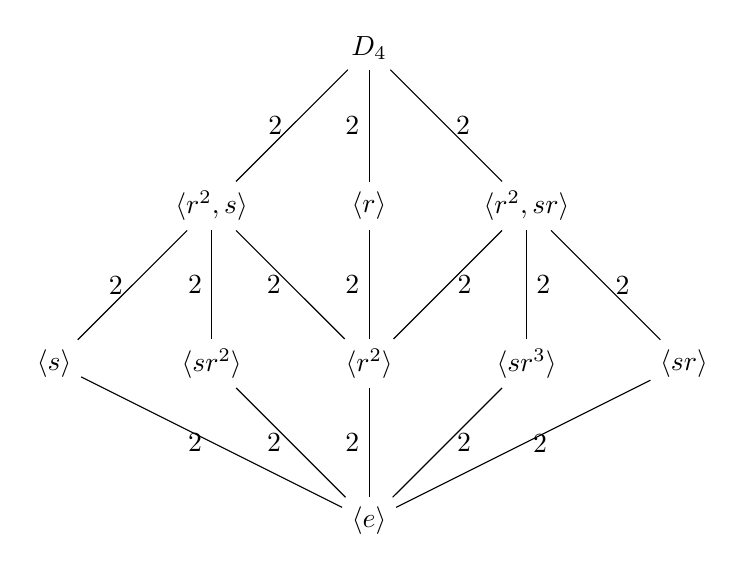
\begin{tikzpicture}[node distance=2cm]
            \node (D4) {$D_4$};
            \node[below of=D4] (r) {$\langle r\rangle$};
            \node[left of=r] (r2s) {$\langle r^2,s\rangle$};
            \node[right of=r] (r2sr) {$\langle r^2,sr\rangle$};
            \node[below of=r] (r2) {$\langle r^2\rangle$};
            \node[left of=r2] (sr2) {$\langle sr^2\rangle$};
            \node[right of=r2] (sr3) {$\langle sr^3\rangle$};
            \node[right of=sr3] (sr) {$\langle sr\rangle$};
            \node[left of=sr2] (s) {$\langle s\rangle$};
            \node[below of=r2] (1) {$\langle e\rangle$};

            \draw (D4) --node[left] {$2$} (r);
            \draw (D4) --node[left] {$2$} (r2s);
            \draw (D4) --node[right] {$2$} (r2sr);
            \draw (r) --node[left] {$2$} (r2);
            \draw (r2s) --node[left] {$2$} (sr2);
            \draw (r2s) --node[left] {$2$} (s);
            \draw (r2s) --node[left] {$2$} (r2);
            \draw (r2sr) --node[right] {$2$} (sr3);
            \draw (r2sr) --node[right] {$2$} (sr);
            \draw (r2sr) --node[right] {$2$} (r2);
            \draw (r2) --node[left] {$2$} (1);
            \draw (sr2) --node[left] {$2$} (1);
            \draw (sr3) --node[right] {$2$} (1);
            \draw (sr) --node[right] {$2$} (1);
            \draw (s) --node[left] {$2$} (1);
        \end{tikzpicture}
        \caption{Diagrama de Hasse para los subgrupos de $D_4$.}
\end{figure}

\noindent
Si consideramos los 5 grupos del centro del diagrama y los dividimos entre $\langle r^2 \rangle $, llegamos a que el conjunto que contiene a estos es isomorfo al grupo de Klein:
    \begin{figure}[H]
        \centering
            \begin{subfigure}{0.45\textwidth}
                    \centering
                    \begin{tikzpicture}[node distance=2cm]
                        \node (D4) {$D_4$};
                        \node[below of=D4] (r) {$\dfrac{\langle r\rangle}{\langle r^2 \rangle }$};
                        \node[left of=r] (r2s) {$\dfrac{\langle r^2,s\rangle}{\langle r^2 \rangle }$};
                        \node[right of=r] (r2sr) {$\dfrac{\langle r^2,sr\rangle}{\langle r^2 \rangle }$};
                        \node[below of=r] (r2) {$\dfrac{\langle r^2\rangle}{\langle r^2 \rangle }$};

                        \draw (D4) --node[left] {} (r);
                        \draw (D4) --node[left] {} (r2s);
                        \draw (D4) --node[right] {} (r2sr);
                        \draw (r) --node[left] {} (r2);
                        \draw (r2s) --node[left] {} (r2);
                        \draw (r2sr) --node[right] {} (r2);
                    \end{tikzpicture}
            \end{subfigure}\hfill
            \begin{subfigure}{0.45\textwidth}
                \centering
                \begin{tikzpicture}[node distance=2cm]
                    \node (V) {$V$};
                    \node (1) [below of=V, xshift=-3cm] {$\left\langle (1\ 2)(3\ 4)\right\rangle$};
                    \node (2) [below of=V] {$\left\langle (1\ 3)(2\ 4)\right\rangle$};
                    \node (3) [below of=V, xshift=3cm] {$\left\langle (1\ 4)(2\ 3)\right\rangle$};
                    \node (4) [below of=2] {$\{1\}$};

                    \draw (V) -- node[above left] {} (1);
                    \draw (V) -- node[left] {} (2);
                    \draw (V) -- node[above right] {} (3);
                    \draw (1) -- node[below left] {} (4);
                    \draw (2) -- node[left] {} (4);
                    \draw (3) -- node[below right] {} (4);
                \end{tikzpicture}    
            \end{subfigure}
    \end{figure}
\end{ejemplo}

\subsubsection{Cuarto Teorema de Isomorfía}
\noindent
Antes de ver el Cuarto Teorema de Isomorfía, hemos de ver dos Lemas previos que nos ayudarán en su demostración:
\begin{lema}[Ley modular o regla de Dedekind]
    Sea $G$ un grupo y $A,B,C < G$ con $A<C$, entonces:
    \begin{equation*}
        A(B\cap C) = AB \cap C
    \end{equation*}
    \begin{proof}
        Por doble implicación:
        \begin{description}
            \item [$\subseteq)$] Sea $z\in A(B\cap C)$, entonces existen $a\in A$ y $x\in B\cap C$ de forma que $z=ax$, con lo que $ax\in AB$ y $ax\in AC = C$ por ser $A<C$, de donde deducimos que $z = ax \in AB\cap C$.
            \item [$\supseteq)$] Sea $z\in AB\cap C$, entonces:
                \begin{itemize}
                    \item Por una parte, como $z\in AB$, tenemos que $\exists a\in A$ y $b\in B$ de forma que $z=ab$.
                    \item Además, como $z\in C$, tenemos que $z = ab \in C$
                \end{itemize}
                Por ser $A<C$, tenemos que $a\in C$, por lo que $a^{-1}\in C$, de donde:
                \begin{equation*}
                    b = a^{-1}z \in C
                \end{equation*}
                Como además teniamos $b\in B$, llegamos a que $z=ab \in A(B\cap C)$.
        \end{description}
    \end{proof}
\end{lema}

\begin{observacion}
    La hipótesis $A<C$ no es necesaria, basta con tener $A\subseteq C$.
\end{observacion}

\begin{lema}\label{lema:4_isomorfia}
    Sea $G$ un grupo y $A,B,C<G$ con $B\lhd A$, entonces:
    \begin{enumerate}
        \item[$i)$] $B\cap C\lhd A\cap C$ y $\nicefrac{A\cap C}{B\cap C} \cong \nicefrac{B(A\cap C)}{B}$.
        \item[$ii)$] Si además $C\lhd G$, entonces: $BC\lhd AC$ y $\nicefrac{AC}{BC}\cong \nicefrac{A}{B(A\cap C)}$
    \end{enumerate}

    \begin{figure}[H]
        \centering
        \begin{tikzpicture}
            \node (G) {$G$};
            \node (A) [below =of G] {$A$};
            \node (C) [below =of G, xshift=-1cm] {$C$};
            
            \node (intersec) [below =of A] {$B(A\cap C)$};
            \node (AintersecC) [below left =of intersec] {$A\cap C$};
            \node (B) [below right =of intersec] {$B$};
            \node (res) [below =of intersec, yshift=-1.5cm] {$B\cap (A\cap C)=B\cap C$};

            \draw (G) -- (A);
            \draw (G) -- (C);
            \draw (A) -- (intersec);
            \draw (A) -- (AintersecC);
            \draw (A) -- node[right] {$\rhd$} (B);
            \draw (C) -- (AintersecC);
            \draw (intersec) -- node[left] {$\rhd$} (B);
            \draw (intersec) -- (AintersecC);
            \draw (AintersecC) -- node[left] {$\rhd$} (res);
            \draw (B) -- (res);
        \end{tikzpicture}
    \end{figure}

    \begin{proof}
        Veamos los dos apartados:
        \begin{enumerate}
            \item[$i)$] Aplicando el Segundo Teorema de Isomorfía sobre el diagrama (observamos el paralelogramo), tenemos el resultado de forma directa:
                \begin{equation*}
                    \nicefrac{A\cap C}{B\cap C} \cong \nicefrac{B(A\cap C)}{B}
                \end{equation*}
            \item[$ii)$] Ahora, si $C\lhd G$ (los elementos de $G$ conmutan con los de $C$), tendremos que $BC = CB$ y $AC = CA$, por lo que $BC, AC < G$. Además, como $B<A$, también tendremos que $BC < AC$. Veamos que esta última relación es normal. Para ello, sean $bc\in BC$, $ax\in AC$:
                \begin{equation*}
                    axbc{(ax)}^{-1} = axbcx^{-1}a^{-1} = axa^{-1}aba^{-1}acx^{-1}a^{-1} = (axa^{-1})(aba^{-1})(acx^{-1}a^{-1})
                \end{equation*}
                Para ver dónde está este último elemento:
                \begin{itemize}
                    \item Como $x\in C$ y $C\lhd G$, $axa^{-1} \in C$.
                    \item Como $b\in B$ y $B\lhd A$, $aba^{-1}\in B$.
                    \item Como $c,x\in C$, tendremos $cx^{-1}\in C$ y por ser $C\lhd G$, $acx^{-1}a^{-1} \in C$.
                \end{itemize}
                En definitiva:
                \begin{equation*}
                    axbc{(ax)}^{-1} \in CBC = BCC = BC
                \end{equation*}
                De donde deducimos que $BC\lhd AC$. Ahora, si tenemos en mente el siguiente diagrama, podemos aplicar el Segundo Teorema de Isomorfía, ya que tenemos $A,BC< AC$ y $BC\lhd AC$.

                \begin{figure}[H]
                    \centering
                    \begin{tikzpicture}
                        \node (HK) {$AC$};
                        \node (H) [below left =of HK] {$A$};
                        \node (K) [below right =of HK] {$BC$};
                        \node (HcapK) [below =of HK, yshift=-1.5cm] {$BC\cap A = B(A\cap C)$};

                        \draw (G) -- (HK);
                        \draw (HK) -- (H);
                        \draw (HK) -- (K);
                        \draw (H) -- (HcapK);
                        \draw (K) -- (HcapK);
                    \end{tikzpicture}
                \end{figure}
                El Segundo Teorema de Isomorfía nos dice que $B(C\cap A)\lhd A$, y que:
                \begin{equation*}
                    \nicefrac{A}{B(A\cap C)} \cong \nicefrac{AC}{BC}
                \end{equation*}
        \end{enumerate}
    \end{proof}
\end{lema}

\begin{observacion}
    Sin embargo, el Lema anterior se podría hacer también suponiendo solo que $A,B\subseteq G$ para $A$ y $B$, solo es necesario suponer que $C<G$.
\end{observacion}

\noindent
A continuación, veremos el Cuarto Teorema de Isomorfía, o Teorema de Zassenhaus, para el cual conviene pensar en la Figura~\ref{fig:4_isomorfia} (aunque en esta figura el retículo de subgrupos está al revés de a lo que estamos acostumbrados: arriba los conjuntos de menor tamaño y debajo los conjuntos mayores).

\begin{figure}[H]
    \centering
    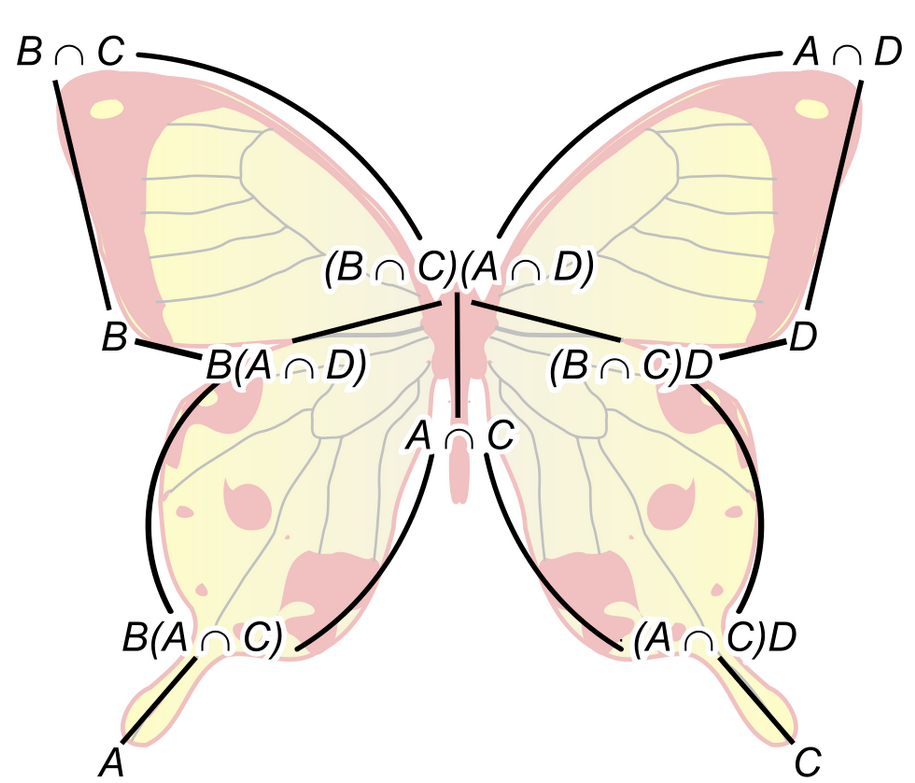
\includegraphics[width=0.8\linewidth]{img/mariposa.png}
    \caption{Situación del Teorema~\ref{teo:4_isomorfia}}
    \label{fig:4_isomorfia}
\end{figure}

% // TODO: NO es necesario aprendérselo
\begin{teo}[Cuarto Teorema de Isomorfía para grupos]\label{teo:4_isomorfia}
    Sea $G$ un grupo y $A_1,C_1,A_2,C_2 < G$ y $C_1\lhd A_1$, $C_2 \lhd A_2$, entonces:
    \begin{enumerate}
        \item[$i)$] $(A_1\cap C_2) C_1 \lhd (A_1 \cap A_2)C_1$.
        \item[$ii)$] $(A_2 \cap C_1) C_2 \lhd (A_1\cap A_2)C_2$.
        \item[$iii)$] $\nicefrac{(A_1\cap A_2)C_1}{(A_1\cap C_2)C_1} \cong \nicefrac{A_1\cap A_2}{(A_1\cap C_2)(A_2\cap C_1)}\cong \nicefrac{(A_1\cap A_2)C_2}{(A_2\cap C_1)C_2} $
    \end{enumerate}

    \begin{proof} Veamos cada apartado:
        \begin{enumerate} % // TODO: El apartado i) lo hizo de otra forma, pero asi tmb vale
            \item[$i)$] En primer lugar\footnote{Esta demostración se hizo en clase de otra forma usando resultados previos. Si alguien hace esta demostración de forma más sencilla que se ponga en contacto con nosotros.}, como $C_1\lhd A_1$, entonces los elementos de $C_1$ conmutarán con los de $A_1$, luego:
                \begin{align*}
                    (A_1\cap C_2)C_1 &= C_1(A_1\cap C_2) \\
                    (A_1\cap A_2)C_1 &= C_1(A_1\cap A_2)
                \end{align*}
                Por lo que ambos serán subgrupos de $G$. Además, como $C_2 < A_2$, tenemos ya que:
                \begin{equation*}
                    (A_1\cap C_2) C_1 < (A_1\cap A_2) C_1
                \end{equation*}
                Para ver la normalidad, sean $x\in (A_1\cap A_2)C_1, y\in (A_1\cap C_2)C_1$, entonces existirán elementos $a\in A_1\cap A_2, b\in A_1\cap C_2, c,c' \in C_1$ de forma que:
                \begin{equation*}
                    x = ac \qquad y = bc'
                \end{equation*}
                Si calculamos:
                \begin{equation*}
                    xyx^{-1} = acbc'c^{-1}a^{-1} = (aca^{-1})(aba^{-1})(ac'a^{-1})(ac^{-1}a^{-1}) 
                \end{equation*}
                Veamos dónde está este elemento:
                \begin{itemize}
                    \item Como $c\in C_1$, $a\in A_1\cap A_2$ y $C_1\lhd A_1$, $aca^{-1} \in C_1$.
                    \item Como $b\in A_1\cap C_2\subseteq C_2$ y $a\in A_1\cap A_2\subseteq A_2$ con $C_2\lhd A_2$, entonces $aba^{-1}\in A_1\cap C_2$.
                    \item Como $c',c\in C_1$, $a\in A_1\cap A_2$ y $C_1\lhd A_1$, $ac'a^{-1}, ac^{-1}a^{-1}\in C_1$.
                \end{itemize}
                En definitva:
                \begin{equation*}
                    xyx^{-1} \in C_1(A_1\cap C_2)C_1C_1 = (A_1\cap C_2)C_1C_1C_1 = (A_1\cap C_2)C_1
                \end{equation*}
                Y concluimos que $(A_1\cap C_2)C_1 \lhd (A_1\cap A_2)C_1$.
            \item[$ii)$] Es análogo, cambiando los papeles de $C_1$ y $C_2$.
            \item[$iii)$] Para el primer isomorfismo, si tomamos:
                \begin{align*}
                    G_1 &= A_1 \\
                    A &= A_1\cap A_2 \\
                    B &= A_1\cap C_2 \\
                    C &= C_1
                \end{align*}
                Nos encontramos en las Hipótesis del Lema~\ref{lema:4_isomorfia}, ya que $A,B,C<G_1$ y $B\lhd A$, por ser $C_2\lhd A_2$. Como además $C\lhd G_1$ por hipótesis, concluimos que:
                \begin{equation*}
                    \nicefrac{AC}{BC} \cong \nicefrac{A}{B(A\cap C)}
                \end{equation*}
                Que en nuestro caso significa:
                \begin{equation*}
                    \nicefrac{(A_1\cap A_2)C_1}{(A_1\cap C_2)C_1} \cong \nicefrac{A_1\cap A_2}{(A_1\cap C_2)(A_1\cap A_2\cap C_1)} = \nicefrac{A_1\cap A_2}{(A_1\cap C_2)(A_2\cap C_1)} 
                \end{equation*}
                Para el segundo, hemos de tomar:
                \begin{align*}
                    G_2 &= A_2 \\
                    A &= A_1\cap A_2 \\
                    B &= A_1\cap C_2 \\
                    C &= C_2
                \end{align*}
        \end{enumerate}
    \end{proof}
\end{teo}

\section{Producto directo}
En un ejemplo del Capítulo~\ref{cap:1} vimos que dados dos grupos $H$ y $G$ podíamos definir de forma sencilla una operación en $H\times G$ en función de las operaciones de $H$ y $G$, que nos dotaba a $H\times G$ de estructura de grupo. A este grupo lo llamábamos grupo directo de $G$ y $H$, grupo que volveremos a definir a partir de ahora y en el que nos centraremos durante esta sección.

\begin{definicion}[Producto directo]
    Sean $H$ y $G$ dos grupos, definimos en el producto cartesiano $H\times G$ la operación
    \Func{\cdot}{(H\times G)\times (H\times G)}{H\times G}{(h,k)(h',k')}{(hh',kk')}
    Se verifica que $H\times G$ junto con esta operación es un grupo:
    \begin{itemize}
        \item Es claro que la operación es asociativa, por ser las respectivas operaciones de $H$ y $G$ asociativas.
        \item El elemento $(1,1)\in H\times G$ es el elemento neutro para la operación.
        \item Dado un elemento $(h,k)\in H\times G$, tenemos que:
            \begin{equation*}
                (h,k)(h^{-1},k^{-1}) = (hh^{-1},kk^{-1}) = (1, 1)
            \end{equation*}
    \end{itemize}
    Este grupo que hemos definido en $H\times G$ recibirá el nombre de \underline{producto directo} de $H$ y $G$.\\

    Algunos autores llaman al producto directo que hemos definido producto directo externo, para diferenciarlo del producto directo interno, que luego definiremos. Sin embargo, nosotros lo llamaremos simplemente producto directo.
\end{definicion}

\begin{prop}
    Si $H$ y $K$ son dos grupos finitos, entonces:
    \begin{enumerate}
        \item[$i)$] $|H\times K| = |H||K|$.
        \item[$ii)$] $O(h,k) = \mcm(O(h), O(k))$ $\forall (h,k)\in H\times K$.
    \end{enumerate}
    \begin{proof}
        Veamos las dos propiedades:
        \begin{enumerate}
            \item[$i)$] Se vió en Álgebra I.
            \item[$ii)$] Como $H$ y $K$ son finitos, también lo será $H\times K$ y como ya vimos en la Proposición~\ref{prop:orden_grupo}, los órdenes de los elementos son finitos, por lo que el enunciado tiene todo el sentido.

                Llamando $m(h,k) = \mcm(O(h),O(k))$, en primer lugar vemos que:
                \begin{equation*}
                    {(h,k)}^{m(h,k)} = \left(h^{m(h,k)},k^{m(h,k)}\right) = (1,1)
                \end{equation*}
                Donde en la primera igualdad hemos usado la definición del producto directo de $H$ y $K$ y en la segunda hemos usado que $O(h)\mid m(h,k)$ y que $O(k)\mid m(h,k)$.

                Ahora, sea $t\in \mathbb{N}\setminus\{0\}$ de forma que ${(h,k)}^{t} = (1,1)$, tenemos entonces que $h^t = 1$ y $k^t = 1$, con lo que $O(h) \mid t$ y $O(k)\mid t$, de donde deducimos que (por definición de mínimo común múltiplo) $m(h,k)\mid t$. \qedhere
        \end{enumerate} 
    \end{proof}
\end{prop}

\begin{definicion}[Proyecciones e inyecciones]
    Dados $H$ y $G$ dos grupos, en el producto directo de $H$ y $G$ podemos definir 4 aplicaciones que nos serán útiles:
    \begin{enumerate}
        \item La proyección en la primera coordenada, $p_1:H\times G\to H$, dada por:
            \begin{equation*}
                p_1(h,k) = h \qquad \forall (h,k)\in H\times G
            \end{equation*}
        \item La proyección en la segunda coordenada, $p_2:H\times G\to G$, dada por:
            \begin{equation*}
                p_2(h,k) = k \qquad \forall (h,k)\in H\times G
            \end{equation*}
        \item La inyección en la primera coordenada, $i_1:H\to H\times G$, dada por:
            \begin{equation*}
                i_1(h) = (h,1) \qquad \forall h\in H
            \end{equation*}
        \item La inyección en la segunda coordenada, $i_2:G\to H\times G$, dada por:
            \begin{equation*}
                i_2(h) = (1,k) \qquad \forall k\in G
            \end{equation*}
    \end{enumerate}
    Aplicaciones que podremos recordar fácilmente observando la Figura~\ref{fig:proyecciones_inyecciones}.
    \begin{figure}[H]
        \centering
        \shorthandoff{""}
        \begin{tikzcd}
        H \arrow[r, "i_1", shift left] & H\times G \arrow[r, "p_2"', shift right] \arrow[l, "p_1", shift left] & G \arrow[l, "i_2"', shift right]
        \end{tikzcd}    
        \shorthandon{""}
        \caption{Diagrama de las proyecciones y las inyecciones.}
        \label{fig:proyecciones_inyecciones}
    \end{figure}
\end{definicion}

\begin{prop}\label{prop:propiedades_proy_iny}
    Se verifica que:
    \begin{enumerate}
        \item Las proyecciones y las inyecciones son homomorfismos de grupos.
        \item $p_1i_1 = id = p_2i_2$ y las aplicaciones $p_1i_2$ y $p_2i_1$ son la aplicación constantemente igual a $1$.
        \item Las proyecciones son sobreyectivas y las inyecciones son inyectivas.
        \item Si tomamos $H' = \{(h,1) \mid h\in H\}$, tenemos que:
            \begin{equation*}
                Im(i_1) = \ker(p_2) = H' \lhd H\times G
            \end{equation*}
            Además, $H'\cong H$.
        \item De la misma forma, si tomamos $G' = \{(1,k) \mid k\in G\}$, tenemos:
            \begin{equation*}
                Im(i_2) = \ker(p_1) = G' \lhd H\times G
            \end{equation*}
            Además, $G'\cong G$.
        \item $H'\cap G' = \{1\}$.
        \item $xy = yx$ para todo $x\in H'$, $y\in G'$.
    \end{enumerate}
    \begin{proof} 
        Veamos cada apartado:
        \begin{enumerate}
            \item Tenemos 4 casos:
                \begin{itemize}
                    \item Para $p_1$, vemos que:
                        \begin{equation*}
                            p_1((h,k)(h',k')) = p_1(hh',kk') = hh' = p_1(h,k)p_1(h',k') \qquad \forall (h,k),(h',k')\in H\times G
                        \end{equation*}
                        Y la demostración para $p_2$ es análoga.
                    \item Para $i_1$, vemos que:
                        \begin{equation*}
                            i_1(hh') = (hh',1) = (h,1)(h',1) = i_1(h)i_1(h') \qquad \forall h,h'\in H
                        \end{equation*}
                        Y la demostración es análoga para $i_2$.
                \end{itemize}
            \item Si los índices coinciden, tenemos que:
                \begin{align*}
                    &(p_1\circ i_1)(h) = p_1(i_1(h)) = p_1(h,1) = h \qquad \forall h\in H \\
                    &(p_2\circ i_2)(k) = p_2(i_2(k)) = p_2(1,k) = k \qquad \forall k\in G 
                \end{align*}
                Y si no coinciden, tenemos:
                \begin{align*}
                    &(p_1\circ i_2)(k) = p_1(i_2(k)) = p_1(1,k) = 1 \qquad \forall k\in G \\
                    &(p_2\circ i_1)(h) = p_2(i_1(h)) = p_2(h,1) = 1 \qquad \forall h\in H
                \end{align*}
            \item Para comprobar que $p_1$ es sobreyectiva, vemos que dada $h\in H$, tenemos que $p_1(h,1) = h$ y para ver que $p_2$ es sobreyectiva, dado $k\in G$, tenemos que $p_2(1,k) = k$.

                Para ver la inyectividad de $i_1$, si dados $h,h'\in H$ de forma que:
                \begin{equation*}
                    (h,1) = i_1(h) = i_1(h') = (h',1)
                \end{equation*}
                De donde deducimos que $h=h'$, por lo que $i_1$ es inyectiva. La demostración para $i_2$ es análoga.
            \item En primer lugar:
                \begin{align*}
                    Im(i_1) &= \{i_1(h) \mid h\in H\} = \{(h,1) \mid h\in H\} \\
                    \ker(p_2) &= \{(h,k)\in H\times G \mid p_2(h,k)=1\} = \{(h,k)\in H\times G \mid k = 1\} \\ &= \{(h,1)\in H\times G\} = \{(h,1)\mid h\in H\}
                \end{align*}
                Además, la igualdad $H' = \ker(p_2)$ nos dice que $H' \lhd H\times G$, gracias a la Proposición~\ref{prop:caracterizacion_normales_homomorfismo}.

            Para ver que $H'\cong H$, en el apartado 1 vimos que $i_1$ era un homomorfismo y aplicando 3 tenemos que, de hecho, es un monomorfismo. Como $Im(i_1) = H'$, la restricción al codominio de $i_1$ a su imagen nos da un isomorfismo entre $H$ y $H'$, con lo que $H'\cong H$.
            \item Vemos que:
                \begin{align*}
                    Im(i_2) &= \{i_2(k) \mid k\in G\} = \{(1,k) \mid k\in G\} \\
                    \ker(p_1) &= \{(h,k)\in H\times G \mid p_1(h,k) = 1\} = \{(h,k)\in H\times G \mid h=1\} \\ &= \{(1,k)\in H\times G\} = \{(1,k)\mid k\in G\}
                \end{align*}
                La igualdad $G' = \ker(p_1)$ nos vuelve a decir que $G' \lhd H\times G$.

                Y finalmente, para ver que $G'\cong G$, tenemos que $i_2$ es un monomorfismo, por lo que la restricción en codominio a su imagen, $Im(i_2) = G'$ nos da un isomorfismo entre $G$ y $G'$.
            \item La igualdad se tiene porque:
                \begin{equation*}
                    H'\cap G' = \{(h,k)\in H\times G \mid k = 1\ \land\ h = 1\} = \{(1,1)\} = \{1\}
                \end{equation*}
            \item Sean $x\in H'$ y $y\in G'$, entonces $\exists h\in H$ y $k\in G$ de forma que $x = (h,1)$ y $y = (1,k)$, de donde:
                \begin{equation*}
                    xy = (h,1)(1,k) = (h,k) = (1,k)(h,1) = yx
                \end{equation*}
        \end{enumerate}
    \end{proof}
\end{prop}

\begin{prop}
    Sean $A$ y $B$ dos grupos, se cumple que:
    \begin{equation*}
        \dfrac{A\times B}{\{1\}\times B} \cong A \qquad \dfrac{A\times B}{A\times \{1\}} \cong B
    \end{equation*}
    \begin{proof}
        En la Proposición superior ya vimos que $\{1\}\times B, A\times \{1\}\lhd A\times B$, por lo que los cocientes del enunciado tienen todo el sentido. Para el primer isomorfismo, si consideramos la proyección en primera coordenada, $p_1:A\times B\to A$ dada por:
        \begin{equation*}
            p_1(x,y) = x \qquad \forall (x,y)\in A\times B
        \end{equation*}
        Y la proyección al cociente $p:A\times B\to (A\times B)/(\{1\}\times B)$ dada por:
        \begin{equation*}
            p(z) = z(\{1\}\times B) \qquad \forall z\in A\times B
        \end{equation*}
        Observando el siguiente diagrama:
        \begin{figure}[H]
            \centering
            \shorthandoff{""}
            \begin{tikzcd}
            A\times B \arrow[r, "p"] \arrow[rd, "p_1"'] & \dfrac{A\times B}{\{1\}\times B} \arrow[d, "\varphi", dashed] \\
                                                        & A                                                            
            \end{tikzcd}
            \shorthandon{""}
        \end{figure}
        Por la Propiedad Universal del grupo cociente, obtenemos que existe un homomorfismo $\varphi:(A\times B)/(\{1\}\times B)\to A$.
        \begin{itemize}
            \item $p_1$ es sobreyectiva, por ser una proyección, por lo que $\varphi$ será sobreyectiva.
            \item Como $\ker(p_1) = \{1\}\times B$, tenemos que $\varphi$ es inyectiva.
        \end{itemize}
        En definitiva, obtenemos el isomorfismo buscado. Para el segundo, basta considerar la proyección al cociente $(A\times B)/(A\times \{1\})$ y la aplicación $p_2$.
    \end{proof}
\end{prop}

\subsection{Caracterización del grupo directo por isomorfismo}

\begin{teo}[Propiedad universal del producto directo]\label{teo:prop_universal_directo}
    Sea $G$ un grupo y sean $f_1:G\to H$, $f_2:G\to K$ dos homomorfismos de grupos, entonces existe un único homomorfismo de grupos $f:G\to H\times K$ tal que $p_1f=f_1$ y $p_2f = f_2$. 

    \noindent
    Es decir, existe un único homomorfismo $f$ que hace conmutar el siguiente diagrama:

    \begin{figure}[H]
        \centering
        \shorthandoff{""}
        \begin{tikzcd}
          & G \arrow[ld, "f_1"'] \arrow[rd, "f_2"] \arrow[d, "f", dashed] &   \\
        H & H\times K \arrow[l, "p_1"] \arrow[r, "p_2"']                  & K
        \end{tikzcd}
        \shorthandon{""}
    \end{figure}

    \begin{proof}
        Definimos $f:G\to H\times K$ dada por:
        \begin{equation*}
            f(x) = (f_1(x), f_2(x)) \qquad \forall x\in G
        \end{equation*}
        \begin{itemize}
            \item Vemos las dos igualdades:
                \begin{align*}
                    (p_1\circ f)(x) &= p_1(f(x)) = p_1(f_1(x), f_2(x)) = f_1(x) \qquad \forall x\in G \\
                    (p_2\circ f)(x) &= p_2(f(x)) = p_2(f_1(x), f_2(x)) = f_2(x) \qquad \forall x\in G
                \end{align*}
            \item Para ver que $f$ es un homomorfismo:
                \begin{multline*}
                    f(xy) = (f_1(xy), f_2(xy)) = (f_1(x)f_1(y), f_2(x)f_2(y))  \\ = (f_1(x),f_2(x))(f_1(y),f_2(y)) = f(x)f(y) \qquad \forall x,y\in G
                \end{multline*}
            \item Sea $g:G\to H\times K$ un homomorfismo de grupos de forma que $p_1g = f_1$ y $p_2g=f_2$, entonces:
                \begin{align*}
                    g(x) = (p_1(g(x)), p_2(g(x))) = (f_1(x), f_2(x)) = f(x) \qquad \forall x\in G
                \end{align*}
                Por lo que $g = f$.
        \end{itemize}
    \end{proof}
\end{teo}

El producto directo es único salvo isomorfismos. Es decir, si hay otro grupo que verifica la propiedad universal de grupo directo, este debe ser isomorfo al grupo directo.
\begin{teo}
    Sea $L$ un grupo y sean $l_1:L\to H$, $l_2:L\to K$ dos homomorfismos de grupos de forma que si $G$ es un grupo y $f_1:G\to H$ y $f_2:G\to K$ son otros dos homomorfismos que cumplen la tesis de la propiedad universal del producto directo para $L$ (es decir, que existe un único homomorfismo $f:G\to L$ de forma que $l_1f=f_1$ y $l_2f = f_2$). Entonces, tendremos que:
    \begin{equation*}
        L\cong H\times K
    \end{equation*}
    La situación es la descrita en el siguiente diagrama:
   \begin{figure}[H]
       \centering
       \shorthandoff{""}
        \begin{tikzcd}
          & L \arrow[rd, "l_2"] \arrow[ld, "l_1"']                         &   \\
        H &                                                               & K \\
          & G \arrow[lu, "f_1"] \arrow[ru, "f_2"'] \arrow[uu, "f", dashed] &  
        \end{tikzcd}
       \shorthandon{""}
   \end{figure}

   \begin{proof}
       En primer lugar, como $l_1:L\to H$ y $l_2:L\to K$ son dos homomorfismos, verifican las hipótesis de la propiedad universal del grupo cociente, por lo que existe un único homomorfismo $l:L\to H\times K$ de forma que:
       \begin{align*}
           p_1l &= l_1 \\
           p_2l &= l_2
       \end{align*}
       \begin{figure}[H]
           \centering
           \shorthandoff{""}
            \begin{tikzcd}
              & L \arrow[rd, "l_2"] \arrow[ld, "l_1"'] \arrow[d, "l", dashed] &   \\
            H & H\times K \arrow[r, "p_2"'] \arrow[l, "p_1"]                  & K
            \end{tikzcd}
           \shorthandon{""}
       \end{figure}
       \noindent
       Ahora, si tomamos $G = H\times K$ y consideramos $p_1:H\times K\to H$ y $p_2:H\times K\to K$, tenemos dos homomorfismos que por hipótesis pueden factorizarse pasando por $L$, es decir, existe un único homomorfismo $p:H\times K\to L$ de forma que:
       \begin{align*}
           l_1p &= p_1 \\
           l_2p &= p_2
       \end{align*}
       \begin{figure}[H]
           \centering
           \shorthandoff{""}
            \begin{tikzcd}
              & L \arrow[rd, "l_2", bend left] \arrow[ld, "l_1"', bend right] \arrow[d, "l", dashed, bend left] &   \\
            H & H\times K \arrow[r, "p_2"'] \arrow[l, "p_1"] \arrow[u, "p", dashed, bend left]                  & K
            \end{tikzcd}
           \shorthandon{""}
       \end{figure}
       \noindent
       Para terminar la demostración, basta ver que $p$ y $l$ son inversos el uno del otro. Para ello, observamos que:
       \begin{align*}
           l_1 &= p_1l = l_1pl \Longrightarrow pl = id_{L} \\
           p_1 &= l_1p = p_1lp \Longrightarrow lp = id_{H\times K}
       \end{align*}
       Concluimos que $p^{-1} = l$, con lo que $p$ y $l$ son isomorfismos y $L\cong H\times K$.
   \end{proof}
\end{teo}

\noindent
Notemos que tanto en la propiedad universal del producto directo como en su unicidad por isomorfismo solo hemos usado las proyecciones $p_1$ y $p_2$. Si consideramos resultados análogos para las inyecciones $i_1$ y $i_2$, estos seguirán siendo ciertos, teniendo que añadir una hipótesis extra:

\begin{teo}[Propiedad universal del producto directo 2]
    Sea $G$ un grupo y $f_1:H\to G$, $f_2:K\to G$ dos homomorfismos de grupos verificando que:
    \begin{equation*}
        f_1(h)f_2(k) = f_2(k)f_1(h) \qquad \forall h\in H, k\in K
    \end{equation*}
    Entonces, existe un único homomorfismo de grupos $f:H\times K\to G$ tal que $fi_1 = f_1$, $fi_2 = f_2$.

    \begin{figure}[H]
        \centering
        \shorthandoff{""}
            \begin{tikzcd}
                                                   & G                                 &                                        \\
            H \arrow[ru, "f_1"] \arrow[r, "i_1"'] & H\times K \arrow[u, "f"', dashed] & K \arrow[lu, "f_2"'] \arrow[l, "i_2"]
            \end{tikzcd}
        \shorthandon{""}
    \end{figure}

    \begin{proof}
        Definimos $f:H\times K\to G$ dada por:
        \begin{equation*}
            f(h,k) = f_1(h)f_2(k) \qquad \forall (h,k)\in H\times K
        \end{equation*}
        \begin{itemize}
            \item Vemos que verifica las dos igualdades:
                \begin{align*}
                    (f\circ i_1)(h) &= f(i_1(h)) = f(h,1) = f_1(h)f_2(1) = f_1(h) \qquad \forall h\in H \\
                    (f\circ i_2)(k) &= f(i_2(k)) = f(1,k) = f_1(1)f_2(k) = f_2(k) \qquad \forall k\in K 
                \end{align*}
            \item Vemos que $f$ es un homomorfismo, ya que dados $(h,k),(h',k')\in H\times K$:
                \begin{multline*}
                    f((h,k)(h',k')) = f(hh',kk') = f_1(hh')f_2(kk') = f_1(h)f_1(h')f_2(k)f_2(k') \\ = f_1(h)f_2(k)f_1(h')f_2(k') = f(h,k)f(h',k')
                \end{multline*}
            \item Sea $g:H\times K\to G$ otro homomorfismo de grupos de forma que $gi_1 = f_1$ y $gi_2 = f_2$, entonces dado $(h,k)\in H\times K$:
                \begin{equation*}
                    g(h,k) = g((h,1)(1,k)) = g(h,1)g(1,k) = g(i_1(h))g(i_2(k)) = f_1(h)f_2(k) = f(h,k)
                \end{equation*} \qedhere
        \end{itemize}
    \end{proof}
\end{teo}

\begin{teo}
   Sea $L$  un grupo y $l_1:H\to L$, $l_2:K\to L$ dos homomorfismos de grupos que verifican que
   \begin{equation*}
       l_1(h)l_2(k) = l_2(k)l_1(h) \qquad \forall h\in H, k\in K
   \end{equation*}
   y que para todo grupo $G$ y para todo par de homomorfismos $f_1:H\to G$ y $f_2:K\to G$ tales que
   \begin{equation*}
       f_1(h)f_2(k) = f_2(k)f_1(h) \qquad \forall h\in H, k\in K
   \end{equation*}
   existe un único homomorfismo $f:L\to G$ tal que $fl_1 = f_1$ y $fl_2 = f_2$, entonces:
   \begin{equation*}
       L \cong H\times K
   \end{equation*}

   \begin{figure}[H]
       \centering
       \shorthandoff{""}
        \begin{tikzcd}
                                               & L \arrow[dd, "f"', dashed] &                                        \\
        H \arrow[ru, "l_1"] \arrow[rd, "f_1"'] &                            & K \arrow[lu, "l_2"'] \arrow[ld, "f_2"] \\
                                               & G                          &                                       
        \end{tikzcd}
       \shorthandon{""}
   \end{figure}

   \begin{proof}
       En primer lugar, por ser $l_1:H\to L$ y $l_2:K\to L$ dos homomorfismos de forma que $l_1(h)l_2(k) = l_2(k)l_1(h)$ $\forall h\in H,k\in K$, tenemos que existe un único homomorfismo $l:H\times K\to L$ de forma que:
       \begin{align*}
           li_1 &= l_1 \\
           li_2 &= l_2
       \end{align*}
       \begin{figure}[H]
           \centering
           \shorthandoff{""}
            \begin{tikzcd}
                                                  & L                                 &                                       \\
            H \arrow[ru, "l_1"] \arrow[r, "i_1"'] & H\times K \arrow[u, "l"', dashed] & K \arrow[lu, "l_2"'] \arrow[l, "i_2"]
            \end{tikzcd}
           \shorthandon{""}
       \end{figure}
       \noindent
       Ahora, si tomamos $G=H\times K$ y consideramos $i_1:H\to H\times K$ y $i_2:K\to H\times K$, tenemos por la Proposición~\ref{prop:propiedades_proy_iny} que $i_1(h)i_2(k) = i_2(k)i_1(h)$ para todo $h\in H$ y para todo $k\in K$, por lo que por hipótesis tenemos que existe un único homomorfismo $i:L\to H\times K$ de forma que: 
       \begin{align*}
           il_1 &= i_1 \\
           il_2 &= i_2 
       \end{align*}
       \begin{figure}[H]
           \centering
           \shorthandoff{""}
            \begin{tikzcd}
                                                             & L \arrow[d, "i"', dashed, bend right]         &                                                   \\
            H \arrow[ru, "l_1", bend left] \arrow[r, "i_1"'] & H\times K \arrow[u, "l"', dashed, bend right] & K \arrow[lu, "l_2"', bend right] \arrow[l, "i_2"]
            \end{tikzcd}
           \shorthandon{""}
       \end{figure}
       Basta ver que $i$ y $l$ son inversos el uno del otro. Para ello, observamos que:
       \begin{align*}
           l_1 &= li_1 = lil_1 \Longrightarrow li = id_{H\times K} \\
           i_2 &= il_2 = ili_2 \Longrightarrow il = id_L
       \end{align*}
       Concluimos que $i^{-1} = l$, con lo que $i$ y $l$ son isomorfismos y $L\cong H\times K$.
   \end{proof}
\end{teo}

\subsection{Producto directo de una familia de grupos}
Los resultados vistos para el producto directo de dos grupos $G$ y $H$ puede generalizarse para el conjunto cartesiano obtenido de multiplicar una familia arbitraria de grupos. Para estudiar este caso, fijaremos la notación en un inicio: sea $\Lambda$ un conjunto arbitrariamente grande, si tenemos una familia de tantos grupos como elementos hay en $\Lambda$:
\begin{equation*}
    \{G_\lm \mid \lm \in \Lambda\}
\end{equation*}
Podemos considerar el producto cartesiano de todos ellos, que denotaremos por $G$:
\begin{equation*}
    G = \prod \{G_\lm \mid \lm \in \Lambda\} = \prod_{\lm \in \Lambda} G_\lm
\end{equation*}

\begin{prop}
    Si $\{G_\lm \mid \lm \in \Lambda\}$ es una familia de grupos, definimos en su producto cartesiano $G = \prod_{\lm\in \Lambda}G_\lm$ la operación $\cdot :G\times G\to G$ dada por:
    \begin{equation*}
        x\cdot y = z
    \end{equation*}
    De forma que la $\lm-$ésima coordenada de $z$ es el producto de la $\lm-$ésima coordenadas de $x$ por la $\lm-$ésima coordenada de $y$. Se verifica que $G$ con esta operación es un grupo.
\end{prop}

\begin{notacion}
    Si $\Lambda = \{1,\ldots,n\}$, notaremos:
    \begin{equation*}
        G = \prod_{\lm \in \Lambda}G_\lm = G_1\times G_2 \times \ldots \times G_n
    \end{equation*}
    Si por otra parte se tiene que $G_\lm = H$ para todo $\lm\in \Lambda$, entonces notaremos:
    \begin{equation*}
        G = \prod_{\lm \in \Lambda}G_\lm = H^\Lambda 
    \end{equation*}
    En el caso de que $\Lambda$ sea finito y tenga $n$ elementos, notaremos $H^n$.
\end{notacion}

\begin{definicion}[Proyecciones e inyecciones]
    Fijado $\lm \in \Lambda$, definimos:
    \begin{itemize}
        \item La proyección en la $\lm-$ésima coordenada, $p_\lm:G\to G_\lm$ dada por:
            \begin{equation*}
                p_\lm(g) = g_\lm \qquad \forall g\in G
            \end{equation*}
            Siendo $g_\lm$ la $\lm-$ésima coordenada de $g$.
        \item La inyección en la $\lm-$ésima coordenada, $i_\lm:G_\lm\to G$ dada por:
            \begin{equation*}
                i_\lm(x) = g \qquad \forall x\in G_\lm
            \end{equation*}
            Donde $g_\mu = 1$ $\forall \mu\in \Lambda\setminus\{\lm\}$ y $g_\lm = x$.
    \end{itemize}
\end{definicion}

\begin{prop}
    Sea $\{G_\lm \mid \lm\in \Lambda\}$ una familia de grupos y sea $G=\prod_{\lm\in \Lambda}G_\lm$, se verifica:
    \begin{enumerate}
        \item $p_\lm$ y $i_\lm$ son homomorfismos de grupos, $\forall \lm\in \Lambda$.
        \item Las proyecciones son epimorfismos y las inyecciones son monomorfismos.
        \item $p_\lm i_\lm = id_{G_\lm}$ y $(p_\lm i_\mu)(x) = 1$ para todo $x\in G_\mu$, $\forall \lm\in \Lambda, \mu \in \Lambda\setminus\{\lm\}$.
        \item $G'_\lm = Im(i_\lm) \cong G_\lm$ y es un subgrupo normal de $G$.
    \end{enumerate}
\end{prop}

\begin{teo}[Propiedad universal del producto directo]
    Sea $\{G_\lm \mid \lm\in \Lambda\}\cup \{H\}$ una familia de grupos y $G=\prod_{\lm\in \Lambda}G_\lm$, si tenemos una familia de homomorfismos para cada coordenada $\{f_\lm :H\to G_\lm \mid \lm\in \Lambda\}$, entonces existe un único homomorfismo $f:H\to G$ de forma que $f_\lm = p_\lm f$, $\forall \lm\in \Lambda$. Además, cualquier otro grupo que verifique esta propiedad será isomorfo a $G$.

    \begin{figure}[H]
        \centering
        \shorthandoff{""}
        \begin{tikzcd}
        H \arrow[d, "f", dashed] \arrow[rd, "f_\lambda"] &           \\
        G \arrow[r, "p_\lambda"]                         & G_\lambda
        \end{tikzcd}
        \shorthandon{""}
    \end{figure}
\end{teo}

\subsection{Producto directo de una familia finita de subgrupos}

\begin{teo}[Ley asociativa general]
    Tenemos que:
    \begin{enumerate}
        \item Si $G_1,G_2,G_3$ son tres grupos, entonces:
            \begin{equation*}
                (G_1\times G_2) \times G_3 \cong G_1 \times G_2 \times G_3 \cong G_1\times (G_2\times G_3)
            \end{equation*}
        \item Si $G_1,G_2,\ldots,G_n$ son $n$ grupos, entonces si $k\in \{1,\ldots,n-1\}$, se tiene:
            \begin{equation*}
                \left(\prod_{j=1}^{k}G_j\right) \times \left(\prod_{j=k+1}^{n}G_j\right) \cong \prod_{j=1}^{n}G_j
            \end{equation*}
    \end{enumerate}
\end{teo}

\begin{teo}
    Sean $G_1,G_2,\ldots,G_n$ $n$ grupos y $G = G_1\times G_2 \times \ldots \times G_n$:
    \begin{enumerate}
        \item $|G| = |G_1| |G_2| \cdots |G_n| $. En particular, $G$ es finito si y solo si $G_k$ es finito, para todo $k\in \{1,\ldots,n\}$.
        \item $O(g_1,\ldots,g_n) = \mcm(O(g_1), \ldots, O(g_n))$, $\forall (g_1,\ldots,g_n)\in G$.
    \end{enumerate}
\end{teo}

\section{Producto directo interno}
El caso que nos interesará ahora será fijado un grupo $G$, consideramos dos subgrupos suyos, $H,K<G$ y trataremos de caracterizar cuándo $H\times K \cong G$. En cuyo caso, diremos que $G$ es \underline{producto directo interno} de $H$ y de $K$.

\begin{definicion}[Conmutador]
    Sea $G$ un grupo, definimos sobre $G$ la operación conmutador $[\cdot ,\cdot ]:G\times G \to G$ dada por:
    \begin{equation*}
        [h,k] = hk{(kh)}^{-1} = hkh^{-1}k^{-1}  \qquad \forall h,k\in G
    \end{equation*}
    Esta operación viene a decirnos cómo de abelianos son los elementos $h$ y $k$ que estemos considerando.
\end{definicion}

\begin{prop}\label{prop:primer_conmutador}
    Sea $G$ un grupo y $h,k\in G$:
    \begin{equation*}
        hk = kh \Longleftrightarrow [h,k] = 1
    \end{equation*}
    \begin{proof}
        Basta observar que:
        \begin{equation*}
            hk = kh \Longleftrightarrow {(hk)}^{-1} = {(kh)}^{-1} \Longleftrightarrow [h,k] = hk{(kh)}^{-1} = 1
        \end{equation*}\qedhere
    \end{proof}
\end{prop}

\noindent
Aunque el siguiente Teorema no nos caracteriza el hecho de que el producto de dos subgrupos de un grupo sea producto directo interno, es el resultado al que comúnmente se le conoce como caracterización del producto directo interno, puesto que viene a decirnos cuándo $H\times K \cong G$ bajo un isomorfismo que se obtiene de una forma muy natural.

Por tanto, diremos que $H\times K$ con $H,K<G$ es producto directo interno de $G$ cuando $H\times K\cong G$ bajo el isomorfismo del siguiente Teorema:

\begin{teo}[Caracterización del producto directo interno]\label{teo:carac_prod_interno}
    Sea $G$ un grupo, $H,K<G$, equivalen:
    \begin{enumerate}
        \item[$i)$] La aplicación $\phi:H\times K\to G$ dada por $\phi(h,k) = hk$ es un isomorfismo.
        \item[$ii)$] $H,K\lhd G$, $HK = G$ y $H\cap K = \{1\}$.
        \item[$iii)$] $hk = kh \quad \forall h\in H, k\in K$, $H\lor K = G$ y $H\cap K = \{1\}$.
        \item[$iv)$] $hk = kh \quad \forall h\in H, k\in K$ y para todo $g\in G$, $\exists_1 h\in H, \exists_1 k\in K$ de forma que $g = hk$. 
    \end{enumerate}
    \begin{proof}
        Veamos las implicaciones:
        \begin{description}
            \item [$i)\Longrightarrow ii)$] Veamos las tres propiedades:
                \begin{itemize}
                    \item Primero que $HK = G$:
                        \begin{description}
                            \item [$\subseteq)$] $HK\subseteq G$ por definición de $HK$.
                            \item [$\supseteq)$] Como $\phi$ es sobreyectiva, dado $g\in G$, existen $h\in H$, $k\in K$ de forma que $g = \phi(h,k) = hk$, lo que nos dice que $G \subseteq  HK$. 
                        \end{description}
                    \item Sea $g\in H\cap K$, entonces $g = \phi(g,1) = \phi(1,g) = g$, pero por ser $\phi$ inyectiva, tenemos que $(g,1)=(1,g)$, de donde $g = 1$.
                    \item Finalmente, para ver que $H,K\lhd G$, basta observar que:
                        \begin{figure}[H]
                            \centering
                            \shorthandoff{""}
                            \begin{tikzcd}
                              & G \arrow[d, "\phi^{-1}", bend left]                                      &   \\
                            H & H\times K \arrow[r, "p_2"] \arrow[l, "p_1"] \arrow[u, "\phi", bend left] & K
                            \end{tikzcd}
                            \shorthandon{""}
                        \end{figure}
                        Para deducir:
                        \begin{align*}
                            \ker(p_2\phi^{-1}) &= \{hk\in G \mid k = 1\} = H \\
                            \ker(p_1\phi^{-1}) &= \{hk\in G \mid h = 1\} = K
                        \end{align*}
                        De donde tenemos que $H,K\lhd G$ (ya que $p_2\phi^{-1}$ y $p_1\phi^{-1}$ son homomorfismos y $H$ y $K$ conciden con sus respectivos núcleos, ver la Proposición~\ref{prop:caracterizacion_normales_homomorfismo}).
                \end{itemize}

            \item [$ii)\Longrightarrow iii)$] Dados $h\in H$ y $k\in K$, veamos que $[h,k] = 1$, de donde deducimos que $hk = kh$:
                \begin{equation*}
                    [h,k] = hkh^{-1}k^{-1} = (hkh^{-1})k^{-1} = h(kh^{-1}k^{-1})
                \end{equation*}
                \begin{itemize}
                    \item Por un lado, como $K$ es normal, tendremos que $hkh^{-1}\in K$, de donde $[h,k] = (hkh^{-1})k^{-1}\in K$. 
                    \item Por otro lado, como $H$ es normal, tendremos también que $kh^{-1}k^{-1} \in H$, de donde $[h,k] = h(kh^{-1}k^{-1}) \in H$.
                \end{itemize}
                En definitiva:
                \begin{equation*}
                    [h,k] \in H\cap K = \{1\} \Longrightarrow hk = kh
                \end{equation*}
                Para la segunda propiedad, basta ver que:
                \begin{equation*}
                    G = HK \subseteq H\lor K \subseteq G
                \end{equation*}
            \item [$iii)\Longrightarrow iv)$] Sea $g\in G$, veamos que se expresa como producto de un elemento de $H$ por otro elemento de $K$. Para ello, como $G = H\lor K$, existirán elementos $\alpha_1,\ldots,\alpha_n \in H\cup K$ de forma que:
                \begin{equation*}
                    g = \alpha_1 \ldots \alpha_n
                \end{equation*}
                Pero como $hk = kh$ para todo $k\in K$ y $h\in H$, podremos conmutar los elementos de forma que lleguemos a:
                \begin{equation*}
                    g = (h_1 \ldots h_m) (k_{m+1} \ldots k_{n}) = hk \in HK
                \end{equation*}
                Para ciertos $h\in H$, $k\in K$.
                Para la unicidad, si $g = h_1k_1 = h_2 k_2$, tenemos que:
                \begin{equation*}
                    h_2^{-1}h_1 = k_2k_1^{-1} \in H\cap K = \{1\} \Longrightarrow h_2 = h_1 \land k_1 = k_2
                \end{equation*}
            \item [$iv)\Longrightarrow i)$] Tenemos para $(h_1,k_1),(h_2,k_2)\in H\times K$ arbitrarios que:
                \begin{equation*}
                    \phi((h_1,k_1)(h_2,k_2)) = \phi(h_1h_2,k_1k_2) = h_1h_2k_1k_2 = h_1k_1h_2k_2 = \phi(h_1,k_1)\phi(h_2,k_2)
                \end{equation*}
                De donde $\phi$ es un homomorfismo. La biyectividad de $\phi$ se debe a que dado $g\in G$, existen unos únicos $h\in H$, $k\in K$ de forma que $g = hk = \phi(h,k)$. \qedhere
        \end{description}
    \end{proof}
\end{teo}

\begin{ejemplo} % // TODO: Ej 18
    Veamos si los siguientes ejemplos son o no un producto interno directo, bajo el isomorfismo natural del Teorema anterior:
    \begin{enumerate}
        \item En $G = \mathbb{R}^\ast$, consideramos $H = \{\pm 1\}$ y $K = \{x\in \mathbb{R} \mid x > 0\}$.

            Sí es producto interno directo, ya que se verifican:
            \begin{itemize}
                \item $G = HK$.
                \item $G$ es abeliano, luego $H,K\lhd G$.
                \item $H\cap K = \{1\}$.
            \end{itemize}
            Y podemos aplicar el Teorema~\ref{teo:carac_prod_interno}.
        \item Sean:
            \begin{align*}
                G &= \left\{\left(\begin{array}{cc}
                    a & b \\
                    0 & c 
                \end{array}\right) \in \GL_2(\mathbb{R})\right\} \\
                H &= \left\{\left(\begin{array}{cc}
                    a & 0 \\
                    0 & c 
                \end{array}\right)\in \GL_2(\mathbb{R})\right\} \\
                K &= \left\{\left(\begin{array}{cc}
                    1 & b \\
                    0 & 1 
                \end{array}\right) \in \GL_2(\mathbb{R})\right\}
            \end{align*}
            Dado un elemento de $G$, podemos escribirlo como un elemento de $HK$:
            \begin{equation*}
                \left(\begin{array}{cc}
                    a & 0 \\
                    0 & c 
                \end{array}\right)\left(\begin{array}{cc}
                    1 & b \\
                    0 & 1 
                \end{array}\right) = \left(\begin{array}{cc}
                    a & ab \\
                    0 & c 
                \end{array}\right)
            \end{equation*}
            Luego $G = HK$. Sin embargo, $hk \neq kh$ para $h\in H$ y $k\in K$, ya que:
            \begin{equation*}
                \left(\begin{array}{cc}
                    1 & b \\
                    0 & 1 
                \end{array}\right) \left(\begin{array}{cc}
                    a & 0 \\
                    0 &  c
                \end{array}\right) = \left(\begin{array}{cc}
                    a & bc \\
                    0 & c 
                \end{array}\right) \neq \left(\begin{array}{cc}
                    a & ab \\
                    0 & c 
                \end{array}\right)
            \end{equation*}
            Por lo que $G$ no es producto directo interno de $H$ y de $K$.
        \item Sea $G = \bb{C}^\ast$, consideramos $H = \{z\in \mathbb{C} \mid |z| = 1\}$ y $K = \mathbb{R}^+$. Por la forma polar de los números complejos, tenemos que $G = HK$:
            \begin{equation*}
                z = \dfrac{z}{|z|}|z| \in HK
            \end{equation*}
            Y como $G$ es abeliano, tenemos que $H,K\lhd G$. Además:
            \begin{equation*}
                H\cap K =\{1\}
            \end{equation*}
    \end{enumerate}
\end{ejemplo}

\noindent
Veamos ahora cómo se comportan los subgrupos con el producto directo:
\begin{prop}\label{prop:monomorfismo_aut}
    Sea $G$ un grupo, $H,K<G$, si $H_1<H$ y $K_1<K$, entonces:
    \begin{enumerate}
        \item $H_1\times K_1 < H\times K$.
        \item Existe un monomorfismo $Aut(H)\times Aut(K)\to Aut(H\times K)$.
    \end{enumerate}
    \begin{proof}
        Veamos que los dos se cumplen:
        \begin{enumerate}
            \item $H_1\times K_1 \subseteq H\times K$. Además, como $H_1<H$ y $K_1<K$, $H_1\times K_1$ va a ser cerrado para el producto, el producto será asociativo, tendrá al elemento $(1,1)$ como neutro y fijado un elemento $(x,y)\in H_1\times K_1$, tendremos que ${(x,y)}^{-1}=(x^{-1},y^{-1})\in H_1\times K_1$, de donde concluimos que $H_1\times K_1 < H\times K$.
            \item Consideramos:
                \Func{\psi}{Aut(H)\times Aut(K)}{Aut(H\times K)}{(\alpha, \beta)}{\psi(\alpha,\beta)}
                Donde $\psi(\alpha,\beta):H\times K \to H\times K$ viene dada por:
                \begin{equation*}
                    \psi(\alpha,\beta)(h,k) = (\alpha(h),\beta(k)) \qquad \forall (h,k)\in H\times K
                \end{equation*}
                Veamos en primer lugar que la aplicación $\psi$ está bien definida, es decir, que $\psi(\alpha,\beta)$ es un automorfismo siempre que $\alpha\in Aut(H)$ y $\beta\in Aut(K)$:
                \begin{itemize}
                    \item Para ver que $\psi(\alpha,\beta)$ es un homomorfismo, dados $(h,k),(h',k')\in H\times K$:
                        \begin{multline*}
                            \psi(\alpha,\beta)((h,k)(h',k')) = \psi(\alpha,\beta)(hh',kk') = (\alpha(hh'), \beta(kk')) \\ = (\alpha(h)\alpha(h'), \beta(k)\beta(k')) = (\alpha(h),\beta(k))(\alpha(h'),\beta(k')) = \psi(\alpha,\beta)(h,k) \psi(\alpha,\beta)(h',k')
                        \end{multline*}
                    \item Para la sobreyectividad, dado $(h,k)\in H\times K$, como $\alpha\in Aut(H)$ y $\beta\in Aut(K)$ son sobreyectivas, existirán $h'\in H$, $k'\in K$ de forma que:
                        \begin{equation*}
                            \alpha(h') = h \qquad 
                            \beta(k') = k
                        \end{equation*}
                        Por lo que:
                        \begin{equation*}
                            \psi(\alpha,\beta)(h',k') = (\alpha(h'),\beta(k')) = (h,k)
                        \end{equation*}
                    \item Para la inyectividad, sean $(h,k),(h',k')\in H\times K$ de forma que:
                        \begin{equation*}
                            (\alpha(h),\beta(k)) = \psi(\alpha,\beta)(h,k) = \psi(\alpha,\beta)(h',k') = (\alpha(h'),\beta(k')) 
                        \end{equation*}
                        De donde deducimos que:
                        \begin{equation*}
                            \alpha(h) = \alpha(h') \qquad \beta(k) = \beta(k')
                        \end{equation*}
                        Pero como $\alpha$ y $\beta$ son inyectivas, tenemos que $h = h'$ y $k = k'$, de donde $(h,k) = (h',k')$.
                \end{itemize}
                Finalmente, veamos que $\psi$ es un monomorfismo:
                \begin{itemize}
                    \item Para ver que es un homomorfismo, dadas ${(\alpha,\beta),(\alpha',\beta')\in Aut(H)\times Aut(K)}$:
                        \begin{equation*}
                            \psi((\alpha,\beta)(\alpha',\beta')) = \psi(\alpha\alpha',\beta\beta') \AstIg \psi(\alpha,\beta)\psi(\alpha',\beta')
                        \end{equation*}
                        Donde en $(\ast)$ se da la igualdad funcional, ya que para $(h,k)\in H\times K$:
                        \begin{align*}
                            \psi(\alpha\alpha',\beta\beta')(h,k) &= ((\alpha\circ\alpha')(h), (\beta\circ\beta')(k)) = (\alpha(\alpha'(h)), \beta(\beta'(k))) \\
                            (\psi(\alpha,\beta)\psi(\alpha',\beta'))(h,k) &= \psi(\alpha,\beta)(\alpha'(h), \beta'(k)) = (\alpha(\alpha'(h)), \beta(\beta'(k)))
                        \end{align*}
                    \item Para ver que $\psi$ es inyectiva, sean $(\alpha,\beta),(\alpha',\beta')\in Aut(H)\times Aut(K)$ de forma que:
                        \begin{equation*}
                            \psi(\alpha,\beta) = \psi(\alpha',\beta')
                        \end{equation*}
                        Entonces:
                        \begin{equation*}
                            (\alpha(h), \beta(k)) = \psi(\alpha,\beta)(h,k) = \psi(\alpha',\beta')(h,k) = (\alpha'(h), \beta'(k)) \quad \forall (h,k)\in H\times K
                        \end{equation*}
                        De donde deducimos que $\alpha = \alpha'$ y que $\beta = \beta'$, por lo que $\psi$ es inyectiva.
                \end{itemize}
                % Esto nos dice que el producto directo de los automorfismos es inyectivo en los automorfismos del producto directo. Nos dice cómo se pueden descomponer los automorfismos.
        \end{enumerate}
    \end{proof}
\end{prop}

% Veamos cuándo podemos hacerlo:
\begin{teo}\label{teo:grupos_finitos_producto}
    Sean $H,K$ dos grupos finitos tales que $\mcd(|H|,|K|) = 1$, entonces: 
    \begin{enumerate}
        \item $\forall L<H\times K$, $\exists_1 H_1<H, K_1<K$ de forma que:
            \begin{equation*}
                L = H_1\times K_1
            \end{equation*}
            Es decir, todo subgrupo de $H\times K$ se descompone de forma única como un subgrupo de $H$ por un subgrupo de $K$.
        \item La aplicación $\psi:Aut(H)\times Aut(K)\to Aut(H\times K)$ de la Proposición~\ref{prop:monomorfismo_aut} es un isomorfismo.
    \end{enumerate}
    \begin{proof}
        Veamos los dos resultados:
        \begin{enumerate}
            \item Sea $L<H\times K$, consideramos:
                \begin{equation*}
                    H_1 = p_1(L) < H \qquad K_1 = p_2(L) < K
                \end{equation*}
                Por la Proposición~\ref{prop:monomorfismo_aut}, tenemos que $H_1\times K_1 < H\times K$, y por la definición de $L$ que $L < H_1\times K_1$, ya que si $(h,k)\in L$:
                \begin{align*}
                    h &= p_1(h,k) \in  H_1 \\
                    k &= p_2(h,k) \in K_1
                \end{align*}
                Basta ver que $H_1\times K_1 < L$.

                \begin{figure}[H]
                 \centering   
                 \shorthandoff{""}
                \begin{tikzcd}
                H \arrow[d, no head] & H\times K \arrow[l, "p_1"] \arrow[r, "p_2"'] \arrow[d, no head] & K \arrow[d, no head] \\
                H_1                  & L                                                               & K_1                 
                \end{tikzcd}
                 \shorthandon{""}
                \end{figure}
                Para ello, si notamos $n = |H|$ y $m = |K|$, por el Teorema de Bezout $\exists r,s\in \mathbb{Z}$ de forma que:
                \begin{equation*}
                    nr + ms = 1
                \end{equation*}
                \begin{itemize}
                    \item En primer lugar, si $h\in H_1$, por su definición y la sobreyectividad de $p_1$, existirá $(h,k)\in L$ de forma que $p_1(h,k) = h$, de donde:
                        \begin{equation*}
                            L \ni {(h,k)}^{ms} = \left(h^{ms}, k^{ms}\right) = \left(h^{1-nr},1\right) = (h,1)
                        \end{equation*}
                        Por lo que: $\{(h,1)\mid h\in H_1\} \subseteq L$.
                    \item Ahora, si $k\in K_1$, por su definición y la sobreyectividad de $p_2$, existirán $(h,k)\in L$ de forma que $p_2(h,k) = k$, de donde:
                        \begin{equation*}
                            K \ni {(h,k)}^{nr} = \left(h^{nr},k^{nr}\right) = (1, k^{1-ms}) = (1,k)
                        \end{equation*}
                        Por lo que: $\{(1,k)\mid k\in K_1\}\subseteq L$.
                \end{itemize}
                Sea ahora $(h,k)\in H_1\times K_1$, tenemos que:
                \begin{equation*}
                    (h,k) = (h,1)(1,k) \in L
                \end{equation*}
                De donde $H_1\times K_1 < L$. Finalmente, la construcción que hemos realizado nos da la unicidad, pues si existen otros subconjuntos $H_2<H$ y $K_2<K$ de forma que $L = H_2\times K_2$, tendríamos que:
                \begin{equation*}
                    H_2 = p_1(L) = H_1 \qquad K_2 = p_2(L) = K_1
                \end{equation*}
            \item Basta ver que $\psi:Aut(H)\times Aut(K)\to Aut(H\times K)$ es sobreyectiva, es decir, que dada $\varphi \in Aut(H\times K)$, podemos encontrar $\alpha\in Aut(H)$ y $\beta\in Aut(K)$ de forma que $\varphi = \psi(\alpha,\beta)$. Para ello, mostraremos el proceso para encontrar $\alpha$ y el proceso para encontrar $\beta$ es análogo. 

                En primer lugar, lo que hacemos es estudiar la imagen por $\varphi$ del conjunto $H\times \{1\} < H\times K$. Como $\varphi$ es un homomorfismo, sabemos que la imagen de $H\times \{1\}$ por $\varphi$ será un subgrupo de $H\times K$, a quien llamaremos $G_1$:
                \begin{equation*}
                    G_1 = \varphi(H\times \{1\}) < H\times K
                \end{equation*}
                Por el apartado 1, sabemos que podemos encontrar únicos $H_1 < H$ y $K_1 < K$ de forma que $G_1 = H_1\times K_1$. Además, por ser $\varphi$ biyectiva, tendremos que:
                \begin{equation*}
                    |H| = |H\times \{1\}| = |H_1\times K_1| = |H_1||K_1|
                \end{equation*}
                Veamos que $|K_1| = 1$. Para ello, si $m = |K_1| \in \mathbb{N}$: 
                \begin{itemize}
                    \item De la igualdad $|H| = |H_1| m$ deducimos que $m$ divide a $|H|$. 
                    \item Como $m = |K_1|$ y $K_1 < K$, por el Teorema de Lagrange tenemos también que $m$ divide a $|K|$.
                \end{itemize}
                Por la definición del máximo común divisor, concluimos que $m$ divide a \newline $\mcd(|H|,|K|) = 1$, de donde $m = 1$ y $K_1 = \{1\}$.

                Finalmente, de la igualdad $|H| = |H_1|$ concluimos que $H = H_1$. Hemos probado que:
                \begin{equation*}
                    \varphi(H\times \{1\}) = H\times \{1\}
                \end{equation*}
                Definimos ahora $\alpha:H\to H$ dada por:
                \begin{equation*}
                    \alpha(h) = p_1(\varphi(i_1(h))) \qquad \forall h\in H
                \end{equation*}
                Está claro que $\alpha$ es un homomorfismo, como composición de homomorfismos.
                \begin{itemize}
                    \item Para la sobreyectividad de $\alpha$, como $\varphi(H\times \{1\}) = H\times \{1\}$, tenemos que:
                        \begin{equation*}
                            \alpha(H) = p_1(\varphi(i_1(H))) = p_1(\varphi(H\times \{1\})) = p_1(H\times \{1\}) = H
                        \end{equation*}
                    \item Para la inyectividad, sean $h_1,h_2\in H$ de forma que:
                        \begin{equation*}
                            p_1(\varphi(h_1,1)) = \alpha(h_1) = \alpha(h_2) = p_2(\varphi(h_2,1))
                        \end{equation*}
                        Como $\varphi(H\times \{1\}) = H\times \{1\}$, sabemos que existirán $h_1',h_2'\in H$ de forma que:
                        \begin{equation*}
                            \varphi(h_1, 1) = (h_1', 1) \qquad \varphi(h_2,1) = (h_2',1)
                        \end{equation*}
                        Por lo que:
                        \begin{equation*}
                            h_1' = p_1(h_1', 1) = p_1(\varphi(h_1,1)) = p_1(\varphi(h_2,1)) = p_1(h_2', 1) = h_2'
                        \end{equation*}
                        De donde concluimos que $\alpha$ es inyectiva.
                \end{itemize}
                De forma análoga a lo que hicimos anteriormente, puede probarse que:
                \begin{equation*}
                    \varphi(\{1\}\times K) = \{1\}\times K
                \end{equation*}
                Y definiendo $\beta:H\times K\to H\times K$ dada por:
                \begin{equation*}
                    \beta(k) = p_2(\varphi(i_2(k))) \qquad \forall k\in K
                \end{equation*}
                Tenemos que $\beta\in Aut(K)$.\\

                Con estos dos automorfismos, veamos que $\psi(\alpha,\beta) = \varphi$:
                \begin{multline*}
                    \psi(\alpha,\beta)(h,k) = (\alpha(h), \beta(k)) = (p_1(\varphi(h,1)), p_2(\varphi(1,k))) \AstIg \varphi(h,k) \\ \forall (h,k)\in H\times K
                \end{multline*}
                Donde en $(\ast)$ hemos usado que existirán $h'\in H$ y $k'\in K$ de forma que:
                \begin{equation*}
                    \varphi(h,1) = (h', 1) \qquad \varphi(1,k) = (1,k')
                \end{equation*}
                Por lo que:
                \begin{multline*}
                     (p_1(\varphi(h,1)), p_2(\varphi(1,k))) = (p_1(h',1), p_2(1,k')) = (h',k') \\ = (h',1)(1,k') = \varphi(h,1)\varphi(1,k) = \varphi(h,k)
                \end{multline*}
        \end{enumerate}
    \end{proof}
\end{teo}

\noindent
El punto 2 de este último Teorema será un resultado que usemos en numerosos ejercicios, sin considerar de forma explícita la aplicación $\psi$ pero usando el isomorfismo $Aut(H)\times Aut(K) \cong Aut(H\times K)$ bajo las hipótesis apropiadas.

\subsection{Producto directo interno de una familia de subgrupos}
\begin{teo}
    Sea $\{G_\lm \mid \lm \in \Lambda\}$ una familia de grupos de forma que para cada $\lm\in \Lambda$ tenemos $H_\lm < G_\lm$, entonces:
    \begin{equation*}
        \prod_{\lm\in \Lambda} H_\lm < \prod_{\lm\in \Lambda} G_\lm
    \end{equation*}
\end{teo}

\begin{teo}
    Sea $\{G_\lm \mid \lm \in \Lambda\}$, entonces existe un monomorfismo
    \begin{equation*}
        \prod_{\lm\in \Lambda}Aut(G_\lm) \longrightarrow Aut\left(\prod_{\lm\in \Lambda} G_\lm\right)
    \end{equation*}
\end{teo}

\subsection{Producto directo interno de una familia finita de subgrupos}
\begin{teo}\label{teo:prod_dir_int_fam}
    Sea $G$ un grupo y $G_1,\ldots,G_n < G$ $n$ subgrupos de $G$, definimos la aplicación $\phi:G_1\times \ldots \times G_n\to G$ dada por:
    \begin{equation*}
        \phi(g_1,\ldots,g_n) = g_1\cdot \ldots \cdot g_n \qquad \forall (g_1,\ldots,g_n)\in G_1\times \ldots \times G_n
    \end{equation*}
    Son equivalentes:
    \begin{enumerate}
        \item[$i)$] $\phi$ es un isomorfismo.
        \item[$ii)$] $G_k\lhd G$ $\forall k\in \{1,\ldots,n\}$, $G_1\ldots G_n = G$ y $(G_1 \ldots G_{k-1}) \cap G_k = \{1\}$ para todo $k\in \{2,\ldots,n\}$.
        \item[$iii)$] $g_k g_h = g_h g_k$ para todo $g_h\in G_h$, $g_k\in G_k$ con $k\neq h$, $G = G_1\lor \ldots \lor G_n$ y $(G_1 \ldots G_{k-1}) \cap G_k = \{1\}$ para todo $k\in \{2,\ldots,n\}$.
        \item[$iv)$] $g_k g_h = g_h g_k$ para todo $g_h\in G_h$, $g_k\in G_k$ con $k\neq h$, y todo elemento $g\in G$ se expresa de manera única como $g= g_1\ldots g_n$ con $g_k \in G_k$ para todo $k \in \{1,\ldots,n\}$.
    \end{enumerate}
\end{teo}

\begin{teo}
    Sean $G_1,\ldots,G_n$ $n$ grupos de forma que sus órdenes son primos relativos dos a dos, si $G = G_1 \times \ldots \times G_n$, entonces:
    \begin{enumerate}
        \item $\exists_1 H_k < G_k$ tal que $L = H_1\times \ldots \times H_k$ para todo $L<G$.
        \item $Aut(G_1)\times \ldots \times Aut(G_n)\cong Aut(G)$.
    \end{enumerate}
\end{teo}

\section{Producto directo de grupos cíclicos}
\begin{notacion}
    Cuando hablemos del producto directo de dos grupos cíclicos, en vez de usar $\times$, usaremos como notación $\oplus$, ya que normalmente usamos la notación aditiva al trabajar con grupos cíclicos.
\end{notacion}

\begin{ejemplo}
    En primer lugar, hemos de tener en cuenta que el producto directo de dos grupos cíclicos no tiene por qué ser en general un grupo cíclico. Veamos varios ejemplos de que no se cumple:
    \begin{enumerate}
        \item Supongamos que $\mathbb{Z}\oplus\mathbb{Z}$ es cíclico. En cuyo caso, tenemos que $\exists (r,s)\in \mathbb{Z}\oplus\mathbb{Z}$ de forma que:
            \begin{equation*}
                \mathbb{Z}\oplus\mathbb{Z} = \langle (r,s) \rangle 
            \end{equation*}
            De donde para $(1,0)\in \mathbb{Z}\oplus\mathbb{Z}$ $\exists n\in \mathbb{Z}$ de forma que:
            \begin{equation*}
                (1, 0) = n(r,s) \Longrightarrow \left\{\begin{array}{l}
                    nr = 1 \\
                    ns = 0
                \end{array}\right. \Longrightarrow \left\{\begin{array}{l}
                    n,r \in \{\pm 1\} \\
                    s = 0 
                \end{array}\right. \Longrightarrow (r,s) = \left\{\begin{array}{l}
                (-1, 0) \\
                (1, 0)
                \end{array}\right.
            \end{equation*}
            Sin embargo, $(0,1)\in \mathbb{Z}\oplus \mathbb{Z}$, por lo que $\exists m\in \mathbb{Z}$ de forma que:
            \begin{equation*}
                (0,1) = m(1,0) \Longrightarrow \left\{\begin{array}{l}
                    m = 0 \\
                    1 = 0
                \end{array}\right.
            \end{equation*}
            Contradicción, por lo que $\mathbb{Z}\oplus \mathbb{Z}$ no es cíclico.
        \item Ahora, supongamos que $\mathbb{Z}_2\oplus\mathbb{Z}_2$ es cíclico, con lo que de la misma forma, $\exists (r,s)\in \mathbb{Z}_2\oplus\mathbb{Z}_2$ de modo que:
            \begin{equation*}
                \mathbb{Z}_2\oplus\mathbb{Z}_2 = \langle (\overline{r},\overline{s}) \rangle 
            \end{equation*}
            Sin embargo:
            \begin{equation*}
                O(\overline{r},\overline{s}) = \mcm(O(\overline{r}),O(\overline{s})) = \left\{\begin{array}{l}
                    1 \Longleftrightarrow \overline{r}=\overline{s}=0 \\
                    2 \Longleftrightarrow \overline{r}\neq0 \lor \overline{s}\neq 0
                \end{array}\right.
            \end{equation*}
            En $\mathbb{Z}_2\oplus\mathbb{Z}_2$ no hay elementos de orden 4, pero:
            \begin{equation*}
                |\mathbb{Z}_2\oplus\mathbb{Z}_2| = 4
            \end{equation*}
            Un grupo de orden 4 que no tiene elementos de orden 4 nunca puede ser cíclico. De hecho, tendremos que $\mathbb{Z}_2\oplus\mathbb{Z}_2\cong V$.
        \item Un ejemplo de dos grupos cíclicos cuyo producto directo es cíclico es:
            \begin{equation*}
                \mathbb{Z}_2\oplus \mathbb{Z}_3
            \end{equation*}
            Que tiene orden $|\mathbb{Z}_2\oplus \mathbb{Z}_3| = |\mathbb{Z}_2||\mathbb{Z}_3| = 6$. Si consideramos $(\overline{1}, \overline{1})$, tenemos que:
            \begin{equation*}
                O(\overline{1},\overline{1}) = \mcm(O(\overline{1}_2), O(\overline{1}_3)) = \mcm(2,3) = 6
            \end{equation*}
            Por lo que $\mathbb{Z}_2 \oplus \mathbb{Z}_3 = \langle (\overline{1},\overline{1}) \rangle $. Notemos que el motivo de que esto haya sucedido es porque 2 y 3 son primos relativos.
    \end{enumerate}
\end{ejemplo}

\begin{prop}\label{prop:carac_prod_finito_ciclicos}
    Si $G$ y $H$ son grupos cíclicos finitos, entonces:
    \begin{equation*}
        G\oplus H \text{\ es cíclico\ } \Longleftrightarrow \mcd(|G|,|H|) = 1
    \end{equation*}
    \begin{proof}
        Veamos las dos implicaciones. Para ello, supongamos que:
        \begin{equation*}
            G = \langle x \rangle,  \quad O(x) = n, \quad H = \langle y \rangle , \quad O(y) = m
        \end{equation*}
        Para ciertos $x\in G$ y $y\in H$.
        \begin{description}
            \item [$\Longleftarrow)$] Si $\mcd(n,m) = 1$, entonces $\mcm(n,m) = nm$, de donde:
                \begin{equation*}
                    O(x,y) = \mcm(O(x), O(y)) = nm = |G||H| = |G\times H|
                \end{equation*}
                Tenemos un grupo de orden $nm$ que contiene a un elemento de orden $nm$, luego $G\times H = \langle (x,y) \rangle $.
            \item [$\Longrightarrow)$] Si $G\oplus H = \langle (a,b) \rangle $, entonces:
                \begin{equation*}
                    O(a,b) = \mcm(O(a), O(b)) = nm = |G||H| = |G\times H|
                \end{equation*}
                Como $O(a) \mid n$ y $O(b) \mid m$, llegamos a que $O(a) = n$ y $O(b) = m$. Finalmente:
                \begin{equation*}
                    \mcd(n,m) = \dfrac{nm}{\mcm(n,m)} = \dfrac{nm}{nm} = 1
                \end{equation*}
        \end{description}
    \end{proof}
\end{prop}

\begin{coro}
    Si $G_1,G_2,\ldots, G_n$ son $n$ grupos cíclicos finitos, entonces:
    \begin{equation*}
        \bigoplus_{k=1}^n G_k \text{\ cíclico} \Longleftrightarrow \mcd(|G_i|,|G_j|) = 1 \quad \forall i,j \in \{1,\ldots,n\}, i\neq j
    \end{equation*}
\end{coro}

\begin{ejemplo}
    Aplicando esta última proposición:
    \begin{itemize}
        \item $\mathbb{Z}_2\oplus\mathbb{Z}_3\oplus\mathbb{Z}_5 \cong \mathbb{Z}_{30}$.
        \item $\mathbb{Z}_2\oplus\mathbb{Z}_2\oplus\mathbb{Z}_3\oplus\mathbb{Z}_5$ no es cíclico.
    \end{itemize}
\end{ejemplo}

\begin{ejemplo} % // TODO: Ejercicio 17
    Podemos demostrar que $S_3$ no es producto directo interno de subgrupos propios. Por reducción al absurdo, si fuera producto directo, como $|S_3| = 6$, tendría un subgrupo de orden 2 y otro de orden 3, ambos isomorfos a $C_2$ y $C_3$. Si tuviera dos subgrupos propios cuyo producto propio fuera él mismo, tendríamos:
    \begin{equation*}
        S_3 \cong C_2\oplus C_3\cong C_6
    \end{equation*}
    Pero $S_3$ no es cíclico, hemos llegado a una contradicción.
\end{ejemplo}

